\documentclass{article}

\usepackage{Sweave}
\begin{document}
\Sconcordance{concordance:seguimento2.tex:seguimento2.Rnw:%
1 2 1 1 0 15 1 1 24 11 0 1 18 12 0 1 2 4 1 1 5 1 2 3 1 1 5 8 0 1 2 3 1 %
1 3 1 2 2 1 1 3 1 2 2 1 1 3 1 2 5 1 1 5 1 2 3 1 1 5 1 2 3 1 1 3 1 2 2 1 %
1 3 1 2 2 1 1 3 1 2 3 1 1 3 1 2 2 1 1 4 1 2 2 1 1 4 1 2 6 1 1 7 1 2 3 1 %
1 5 8 0 1 2 2 1 1 3 1 2 2 1 1 3 1 2 2 1 1 3 1 2 5 1 1 5 1 2 3 1 1 5 1 2 %
3 1 1 3 1 2 2 1 1 3 1 2 2 1 1 3 1 2 3 1 1 5 1 2 2 1 1 4 1 2 2 1 1 4 1 2 %
6 1 1 7 1 2 3 1 1 5 8 0 1 2 2 1 1 3 1 2 2 1 1 3 1 2 2 1 1 3 1 2 5 1 1 5 %
1 2 3 1 1 5 1 2 3 1 1 3 1 2 2 1 1 3 1 2 2 1 1 3 1 2 3 1 1 5 1 2 2 1 1 4 %
1 2 2 1 1 4 1 2 6 1 1 5 1 2 6 1 1 7 1 2 3 1 1 5 8 0 1 2 2 1 1 3 1 2 2 1 %
1 3 1 2 2 1 1 3 1 2 5 1 1 5 1 2 3 1 1 5 1 2 5 1 1 3 1 2 2 1 1 3 1 2 3 1 %
1 5 1 2 2 1 1 4 1 2 6 1 1 7 1 2 3 1 1 5 8 0 1 2 2 1 1 3 1 2 2 1 1 3 1 2 %
2 1 1 3 1 2 5 1 1 5 1 2 3 1 1 5 1 2 5 1 1 3 1 2 2 1 1 3 1 2 3 1 1 5 1 2 %
2 1 1 4 1 2 4 1 1 7 1 2 3 1 1 5 8 0 1 2 3 1 1 3 1 2 2 1 1 3 1 2 2 1 1 3 %
1 2 5 1 1 5 1 2 2 1 1 5 1 2 5 1 1 3 1 2 2 1 1 3 1 2 3 1 1 5 1 2 3 1 1 4 %
1 2 4 1 1 7 1 2 3 1 1 5 8 0 1 2 3 1 1 3 1 2 2 1 1 3 1 2 2 1 1 3 1 2 5 1 %
1 5 1 2 2 1 1 5 1 2 5 1 1 3 1 2 2 1 1 3 1 2 3 1 1 5 1 2 3 1 1 4 1 2 4 1 %
1 7 1 2 3 1 1 5 8 0 1 2 3 1 1 3 1 2 2 1 1 3 1 2 2 1 1 3 1 2 5 1 1 5 1 2 %
2 1 1 5 1 2 5 1 1 3 1 2 2 1 1 3 1 2 3 1 1 5 1 2 2 1 1 4 1 2 2 1}

\title{PROMSACE: Seguimiento de encuestas}
\author{Hernan Nuñez}
\date{\today}
\maketitle
\begin{abstract}
Lo mostrado en este documento nos da una vision descriptiva y exploratoria sobre los cambios a traves del tiempo (del 28 febrero al 30 de junio) de las encuestas recopiladas y completas. Se trabajo con Latex y RStudio. Pueden encontrar el codigo en https://github.com/HernanPerci/PROMSACE
\end{abstract}

\tableofcontents

\section{Introduccion}
La encuesta sobre la que se respalda el presente informe aun se esta recolectando mediante la platafoma surveymonkey.

\section{bases de datos usadas}
\begin{Schunk}
\begin{Soutput}
Rows: 248
Columns: 6
$ Fecha     <dttm> 2020-02-28, 2020-02-29, 2020-03-01, 2020-03-02, 2020-03-...
$ Mes       <fct> Febrero, Febrero, Marzo, Marzo, Marzo, Marzo, Marzo, Marz...
$ Dia       <fct> viernes, sabado, domingo, lunes, martes, miercoles, jueve...
$ Tipo      <fct> Recopilada, Recopilada, Recopilada, Recopilada, Recopilad...
$ Recuento  <dbl> 142, 24, 16, 143, 149, 68, 44, 90, 13, 8, 222, 228, 300, ...
$ Acumulado <dbl> 142, 166, 182, 325, 474, 542, 586, 676, 689, 697, 919, 11...
\end{Soutput}
\end{Schunk}
\begin{Schunk}
\begin{Soutput}
Rows: 124
Columns: 7
$ Fecha                   <dttm> 2020-02-28, 2020-02-29, 2020-03-01, 2020-0...
$ `Recuento Recopiladas`  <dbl> 142, 24, 16, 143, 149, 68, 44, 90, 13, 8, 2...
$ `Acumulado Recopiladas` <dbl> 142, 166, 182, 325, 474, 542, 586, 676, 689...
$ `Recuento Completas`    <dbl> 119, 18, 10, 125, 124, 57, 38, 79, 10, 8, 2...
$ `Acumulado Completas`   <dbl> 119, 137, 147, 272, 396, 453, 491, 570, 580...
$ Dia                     <fct> viernes, sabado, domingo, lunes, martes, mi...
$ Mes                     <fct> Febrero, Febrero, Marzo, Marzo, Marzo, Marz...
\end{Soutput}
\end{Schunk}

\section{Panorama general del 28 Febrero al 30 de Junio}
\subsection{Graficos de lineas}
Se muestran los cambios de la recoleccion de encuestas recopiladas y completas a lo largo del periodo 28 de febrero al 30 de junio

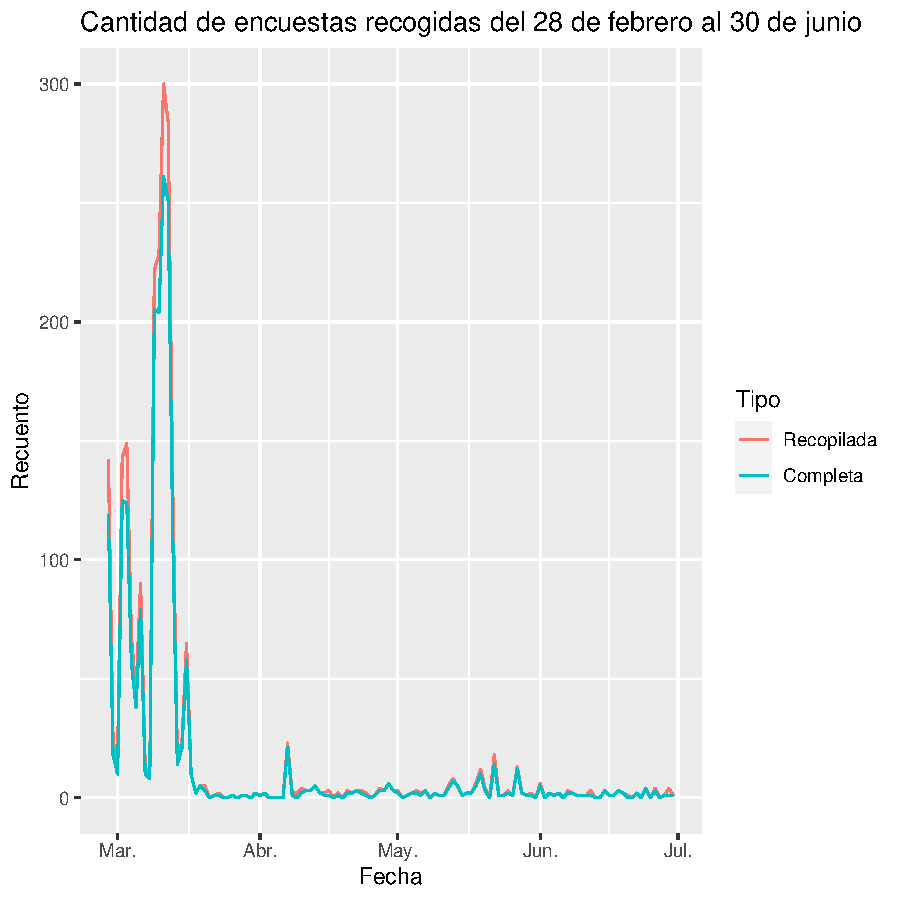
\includegraphics{seguimento2-004}

\subsection{Graficos de barras}
Se comparan las estadisticas de las encuestas recopiladas y completas a lo largo del periodo 28 de febrero al 30 de junio

\begin{Schunk}
\begin{Soutput}
# A tibble: 2 x 4
  Tipo       minimo mediana maximo
  <fct>       <dbl>   <dbl>  <dbl>
1 Recopilada      0       2    300
2 Completa        0       2    261
\end{Soutput}
\end{Schunk}

\subsubsection{Minimo}
El valor es de cero para recopiladas y completas

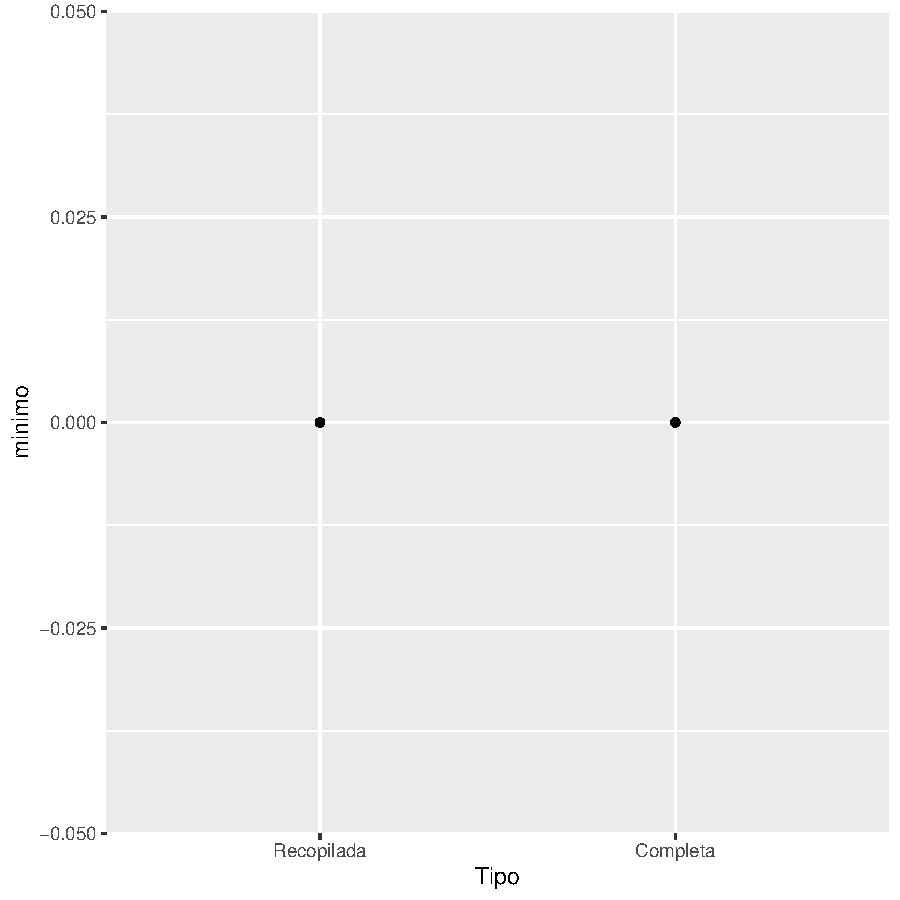
\includegraphics{seguimento2-006}

\subsubsection{Mediana}

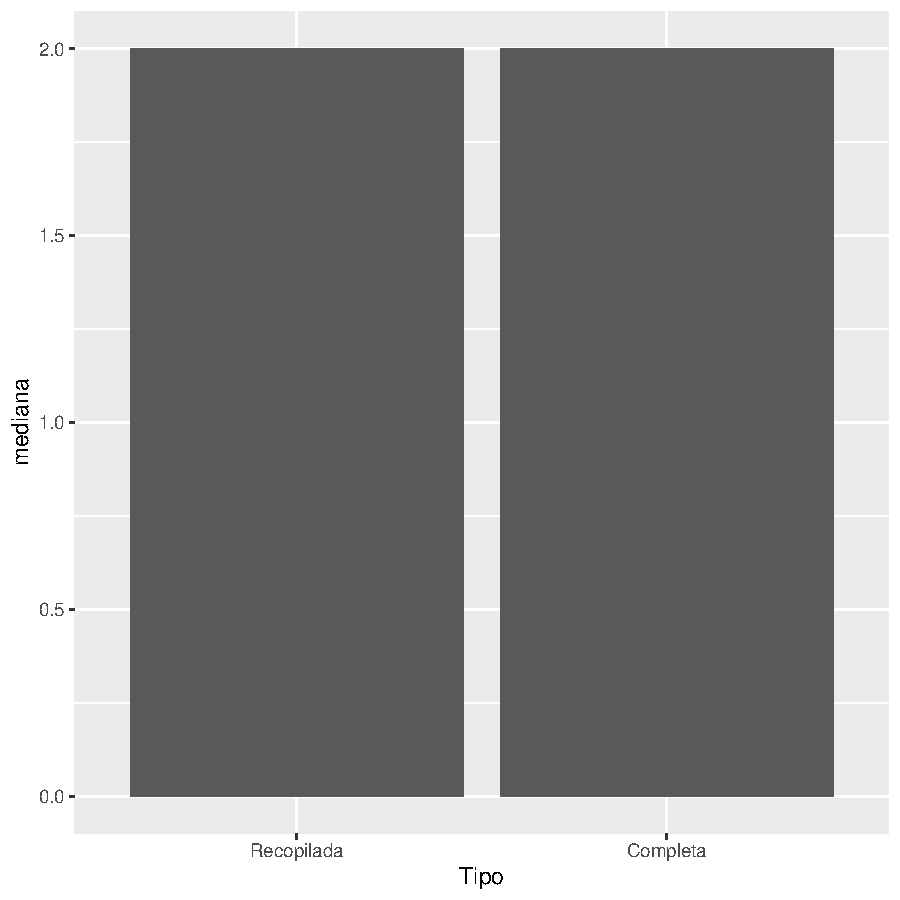
\includegraphics{seguimento2-007}

\subsubsection{Maximo}

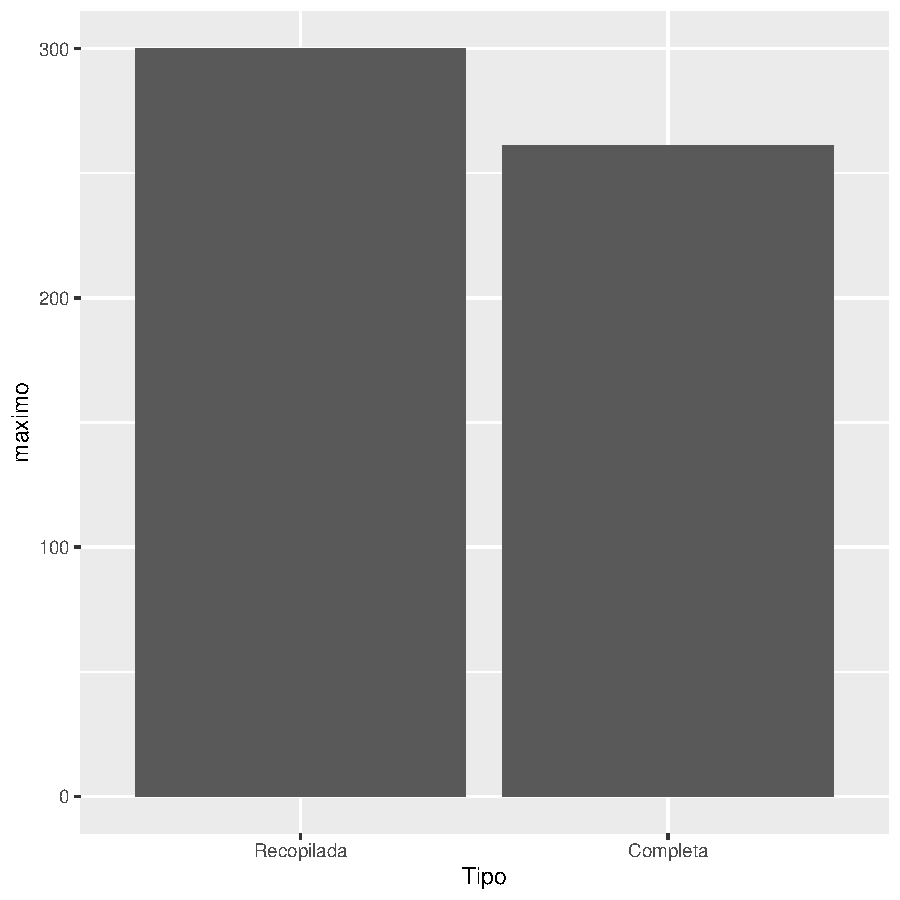
\includegraphics{seguimento2-008}

\subsection{Histogramas}
Se mostraran las distribuciones de las encuestas recopiladas y completas a lo largo del periodo 28 de febrero al 30 de junio

\subsubsection{Recopilada}

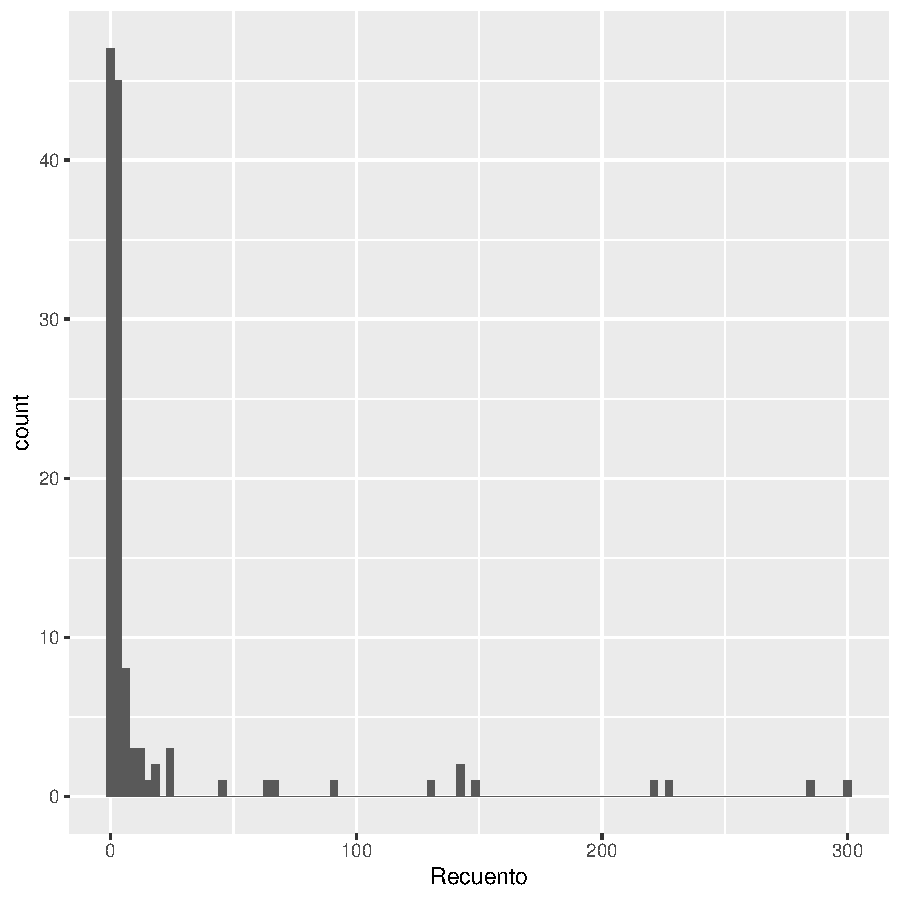
\includegraphics{seguimento2-009}


\subsubsection{Completa}

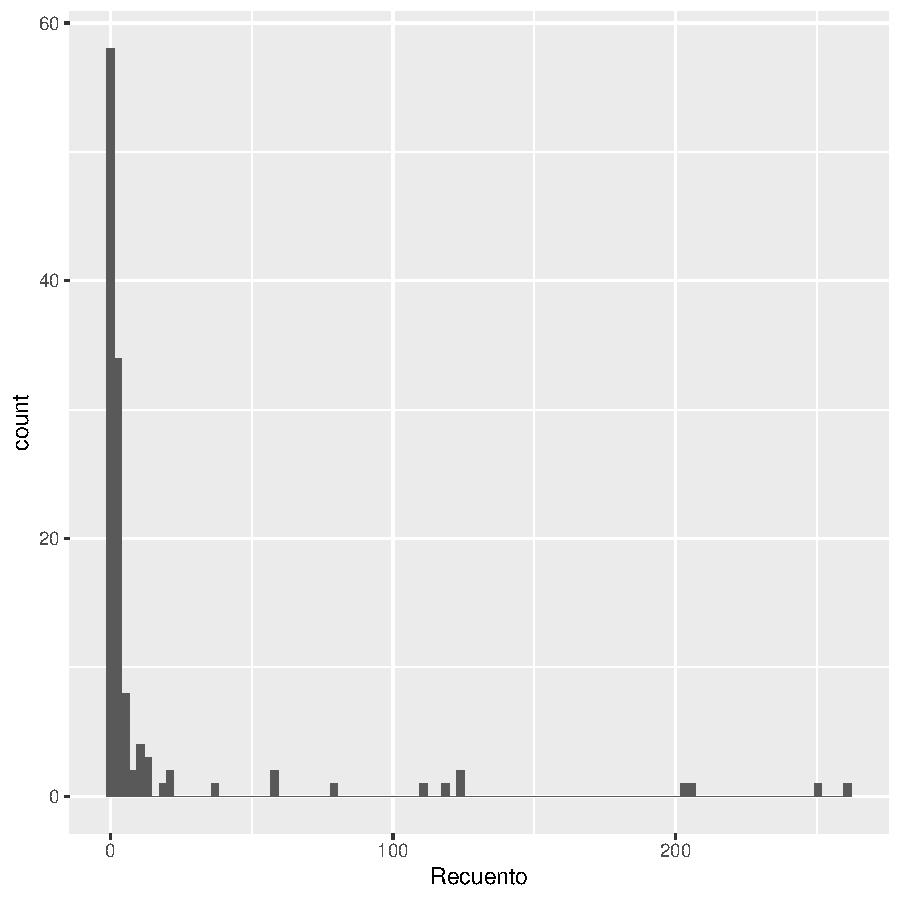
\includegraphics{seguimento2-010}

\subsection{Graficos de cajas}
Se comparan las distribuciones de las encuestas recopiladas y completas a lo largo del periodo 28 de febrero al 30 de junio

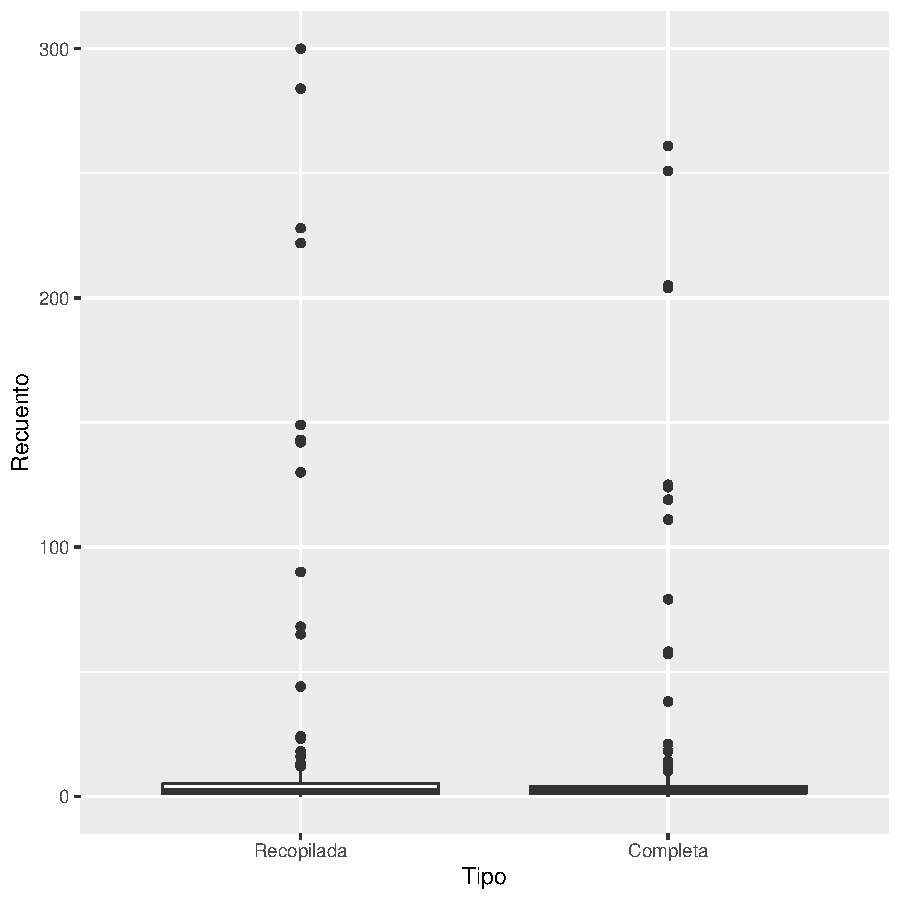
\includegraphics{seguimento2-011}

\subsubsection{Por meses}

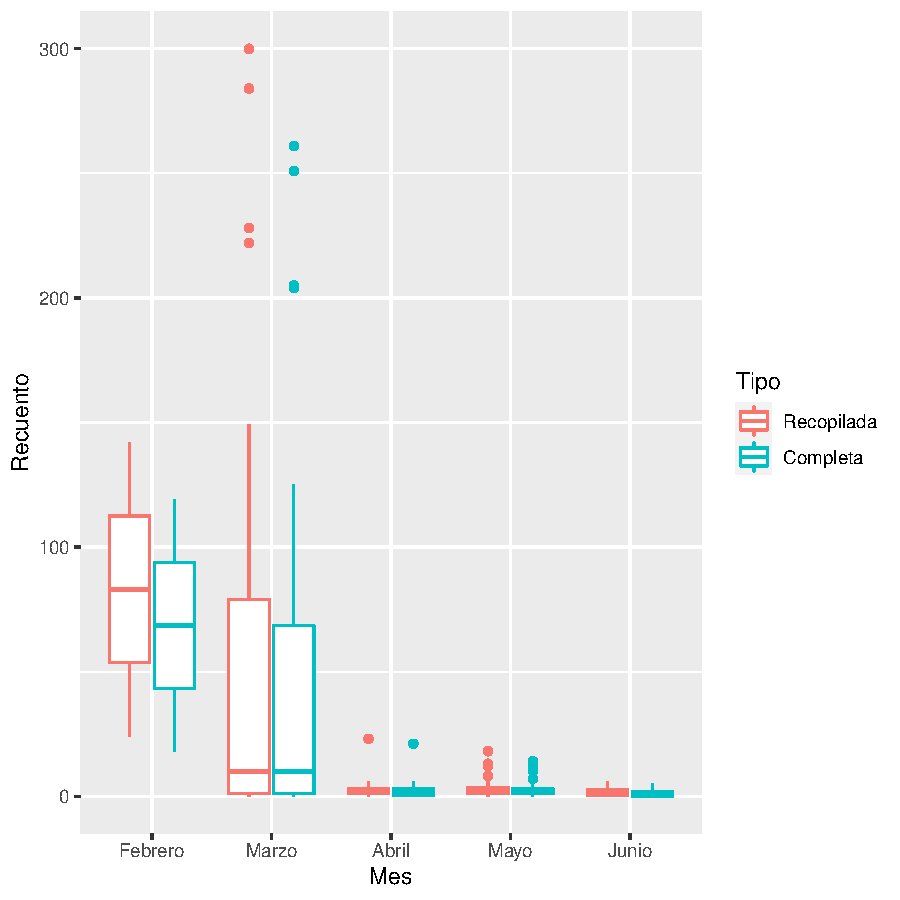
\includegraphics{seguimento2-012}

\subsubsection{Por dia de la semana}

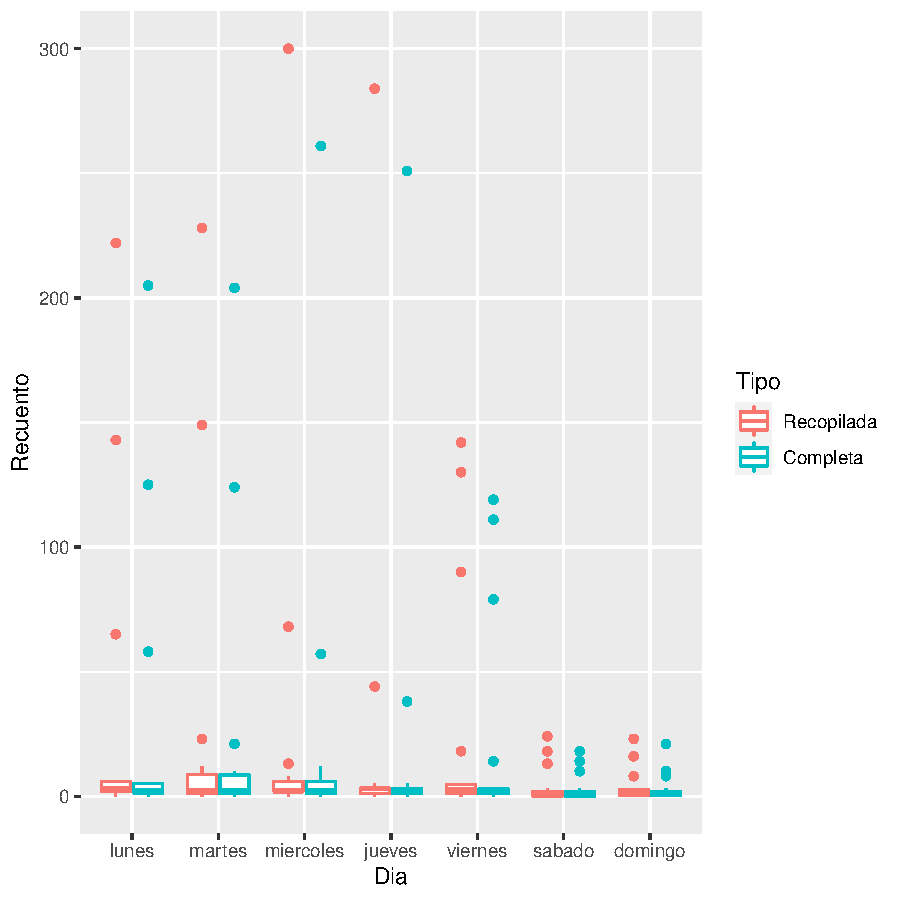
\includegraphics{seguimento2-013}

\subsection{Graficos de puntos}
Se mostraran las posibles relaciones entre las encuestas recopiladas y completas a lo largo del periodo 28 de febrero al 30 de junio

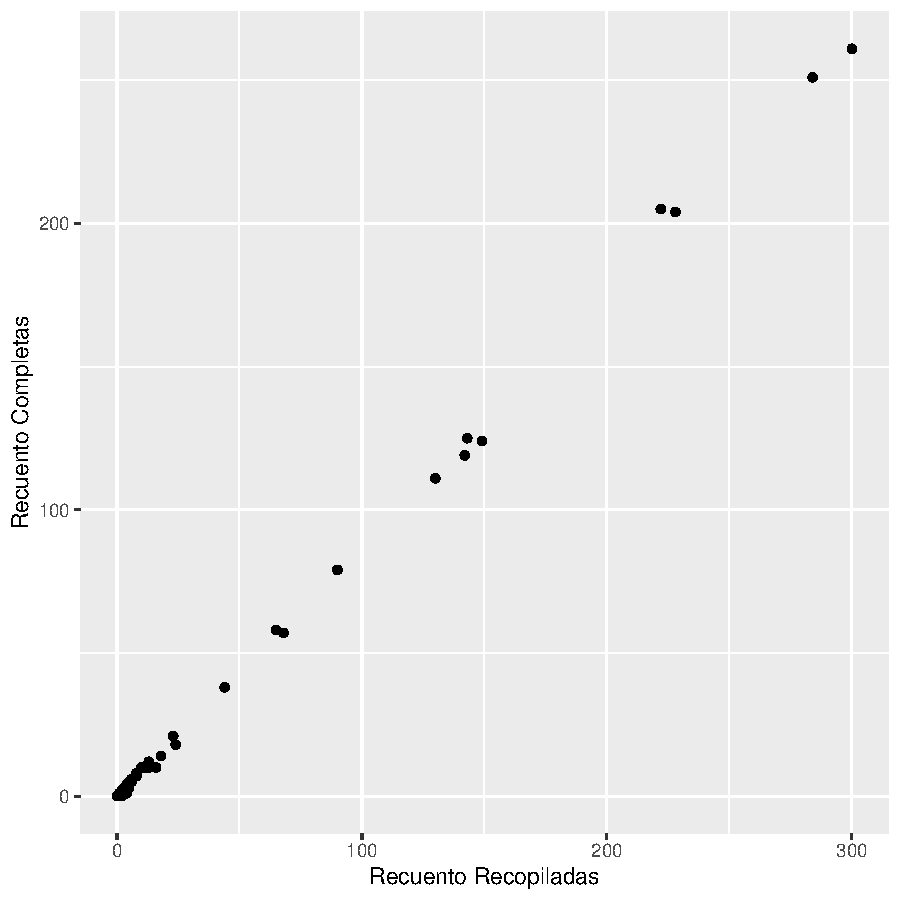
\includegraphics{seguimento2-014}

\subsubsection{Por meses}

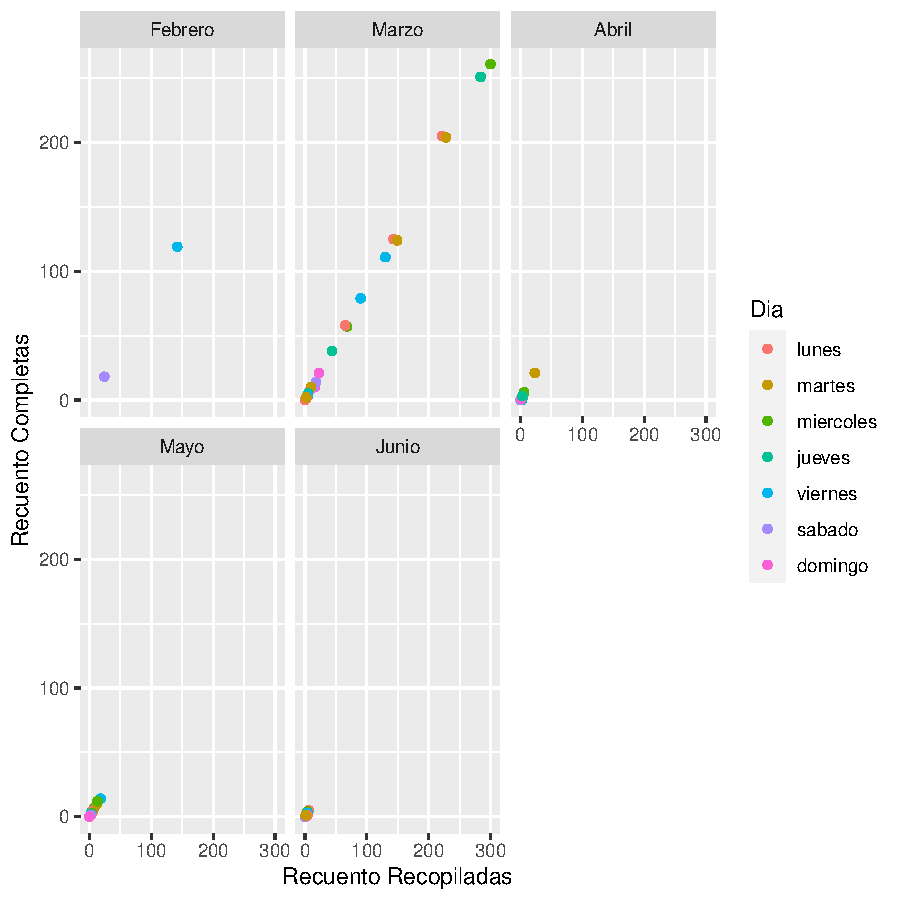
\includegraphics{seguimento2-015}

\subsubsection{Por dias}

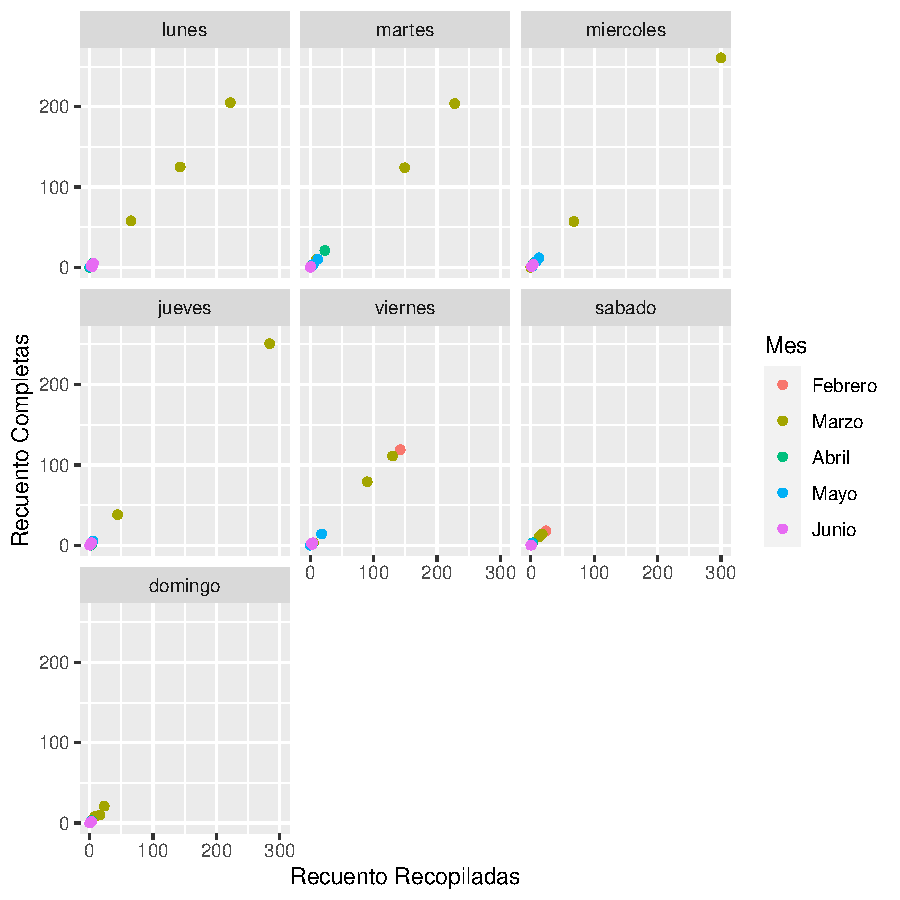
\includegraphics{seguimento2-016}

\section{Panorama antes del covid}
Esta etapa incluye desde el 28 de febrero hasta el 15 de marzo

\subsection{Graficos de lineas}
Se muestran los cambios de la recoleccion de encuestas recopiladas y completas a lo largo del periodo 28 de febrero al 15 de marzo

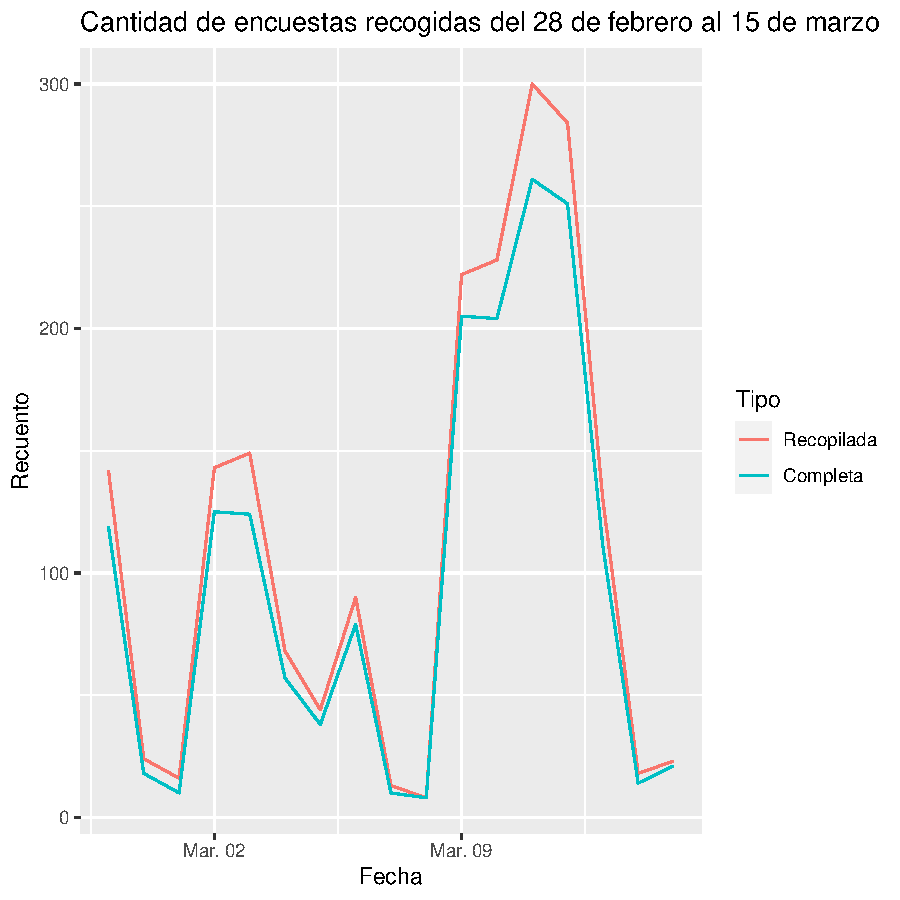
\includegraphics{seguimento2-017}

\subsection{Graficos de barras}
Se comparan las estadisticas de las encuestas recopiladas y completas a lo largo del periodo 28 de febrero al 15 de marzo

\begin{Schunk}
\begin{Soutput}
# A tibble: 2 x 4
  Tipo       minimo mediana maximo
  <fct>       <dbl>   <dbl>  <dbl>
1 Recopilada      8      90    300
2 Completa        8      79    261
\end{Soutput}
\end{Schunk}

\subsubsection{Minimo}

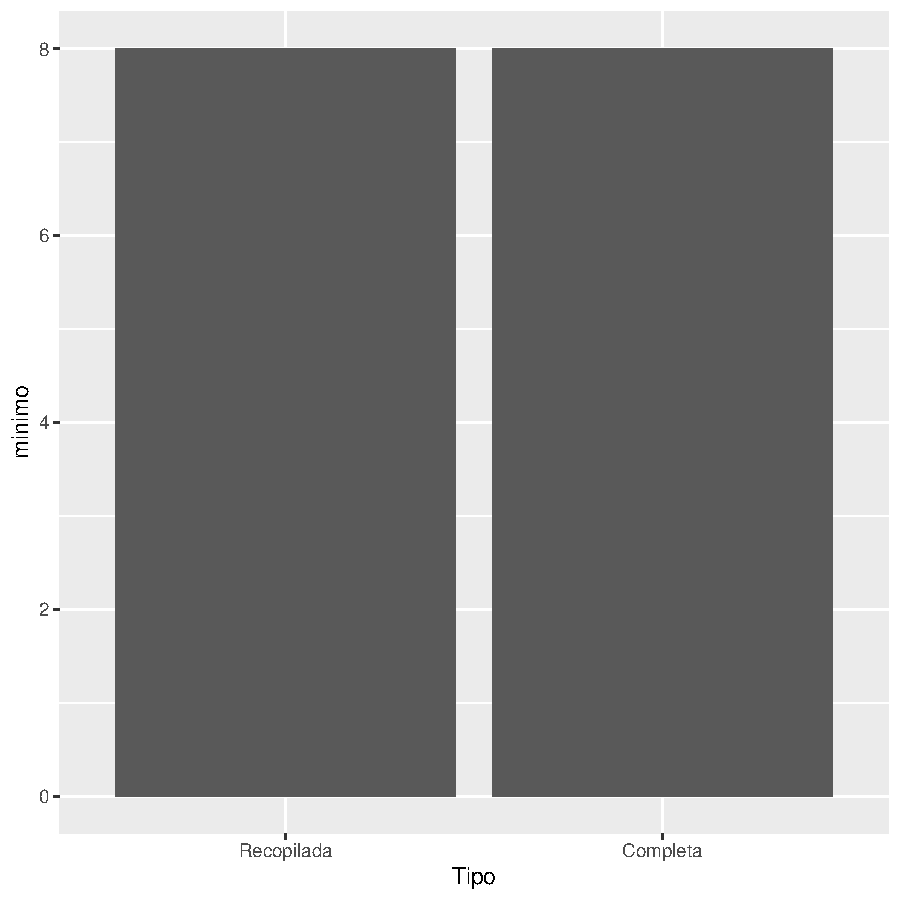
\includegraphics{seguimento2-019}

\subsubsection{Mediana}

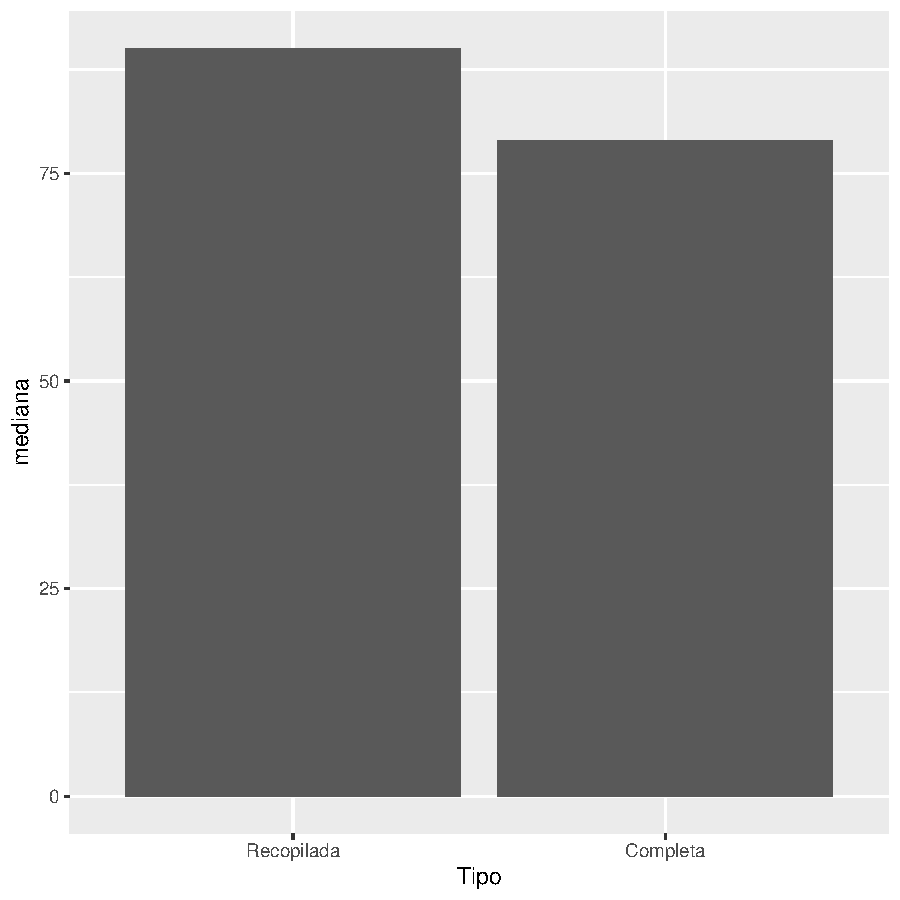
\includegraphics{seguimento2-020}

\subsubsection{Maximo}

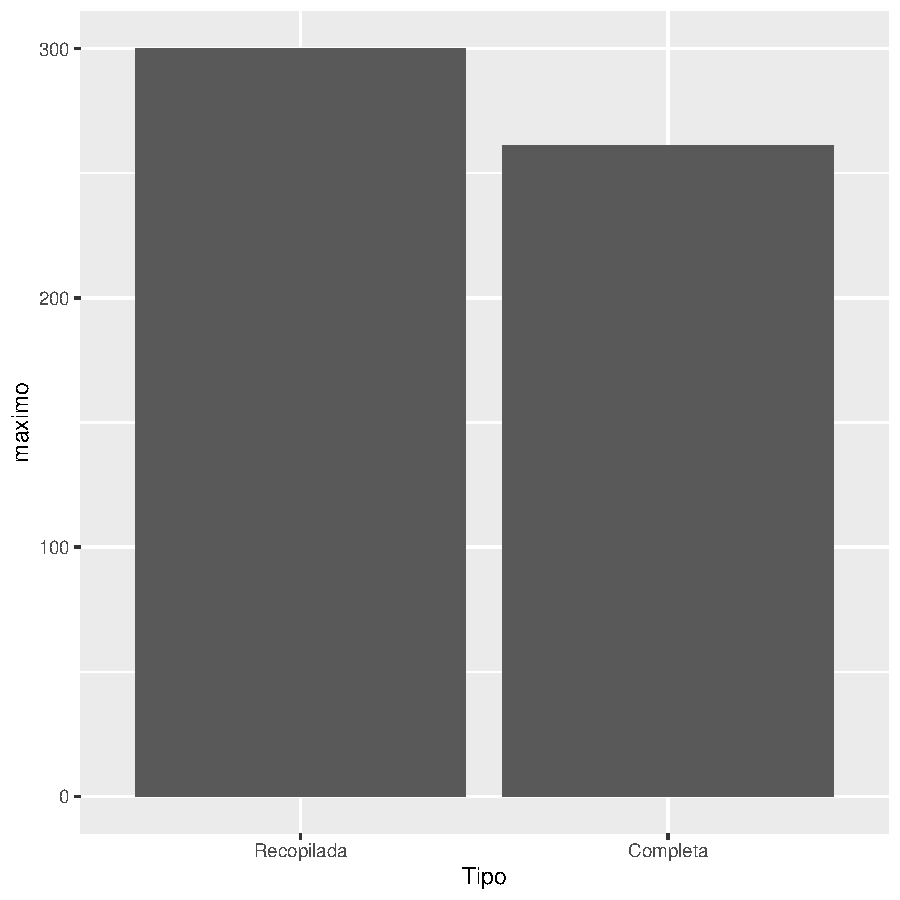
\includegraphics{seguimento2-021}

\subsection{Histogramas}
Se mostraran las distribuciones de las encuestas recopiladas y completas a lo largo del periodo 28 de febrero al 15 de marzo

\subsubsection{Recopilada}

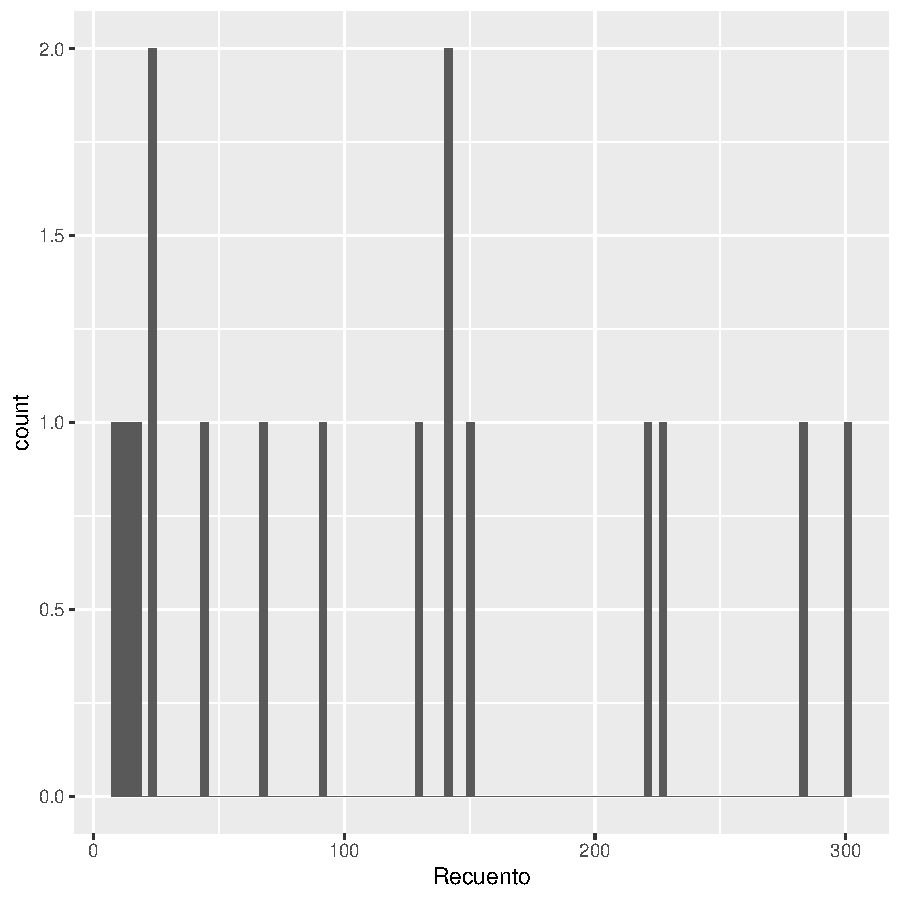
\includegraphics{seguimento2-022}


\subsubsection{Completa}

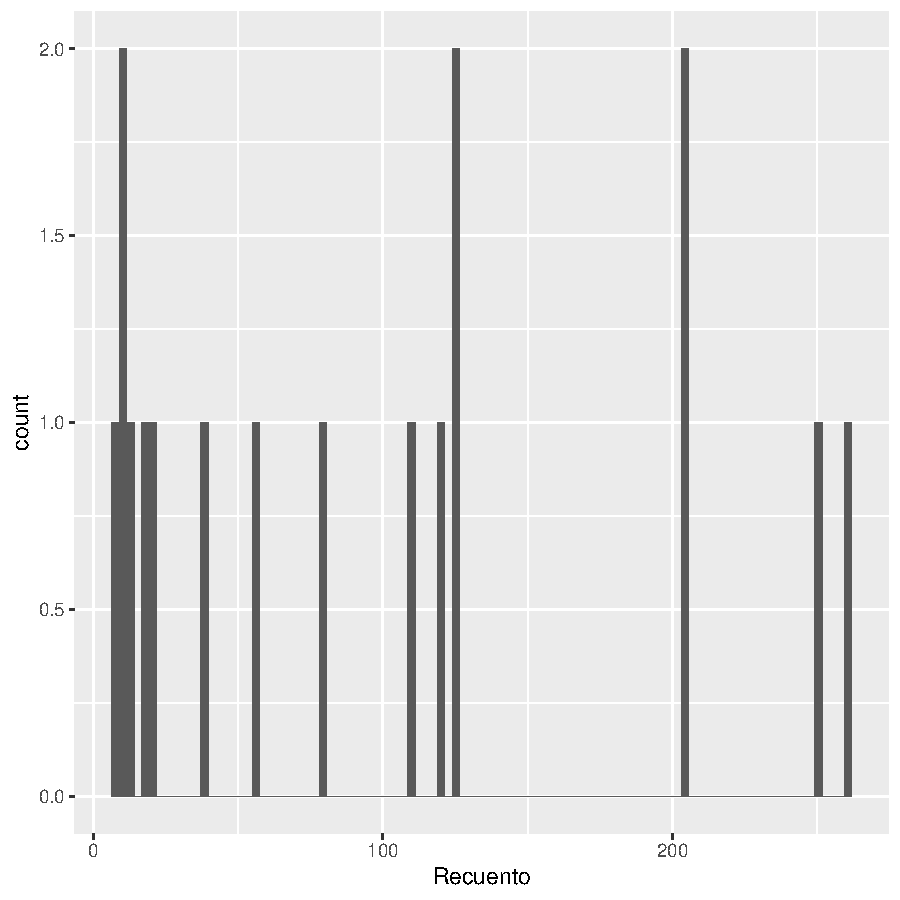
\includegraphics{seguimento2-023}

\subsection{Graficos de cajas}
Se comparan las distribuciones de las encuestas recopiladas y completas a lo largo del periodo 28 de febrero al 15 de marzo

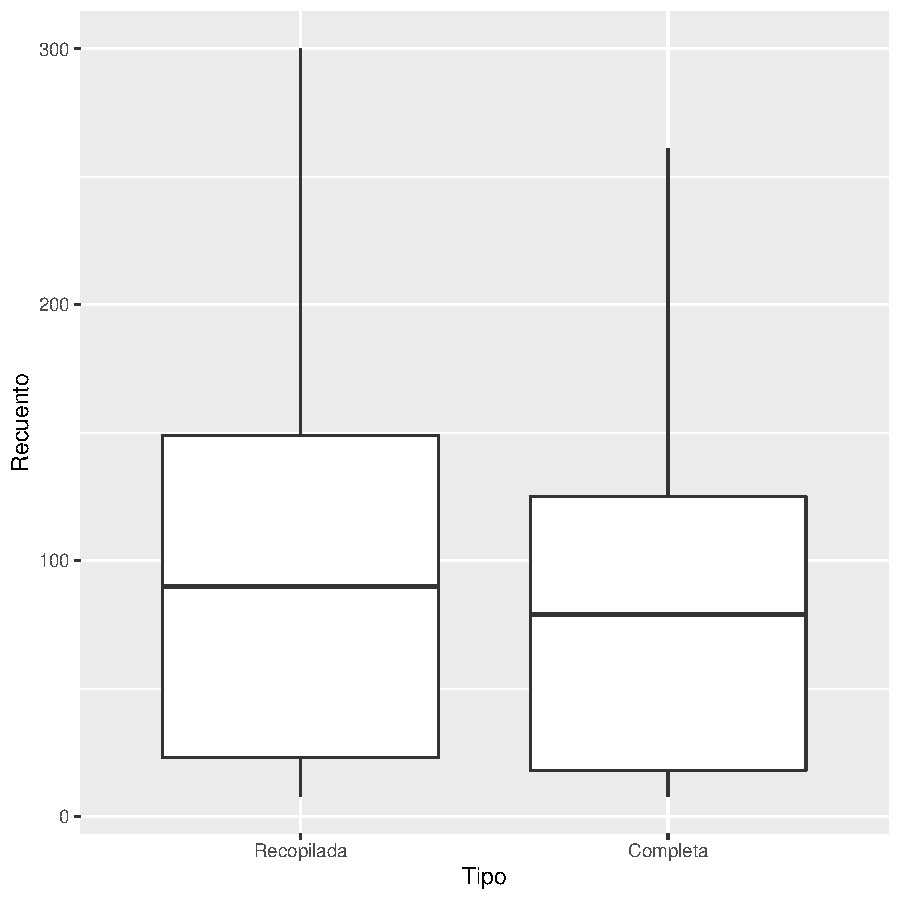
\includegraphics{seguimento2-024}

\subsubsection{Por meses}

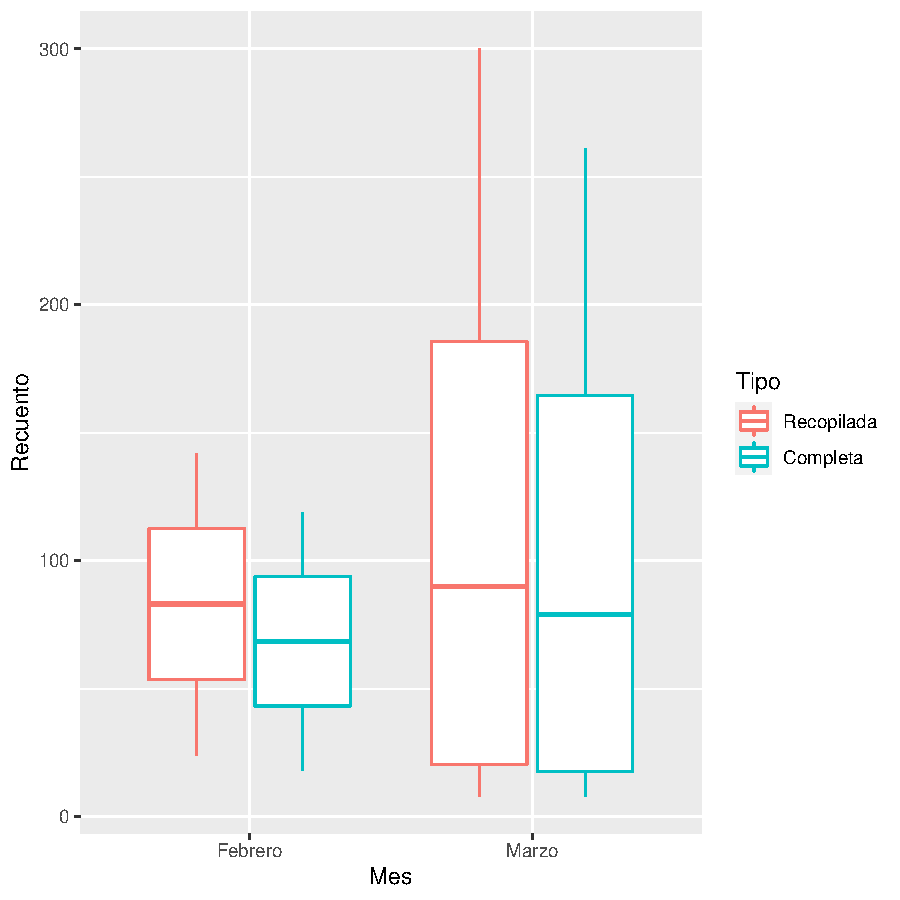
\includegraphics{seguimento2-025}

\subsubsection{Por dia de la semana}

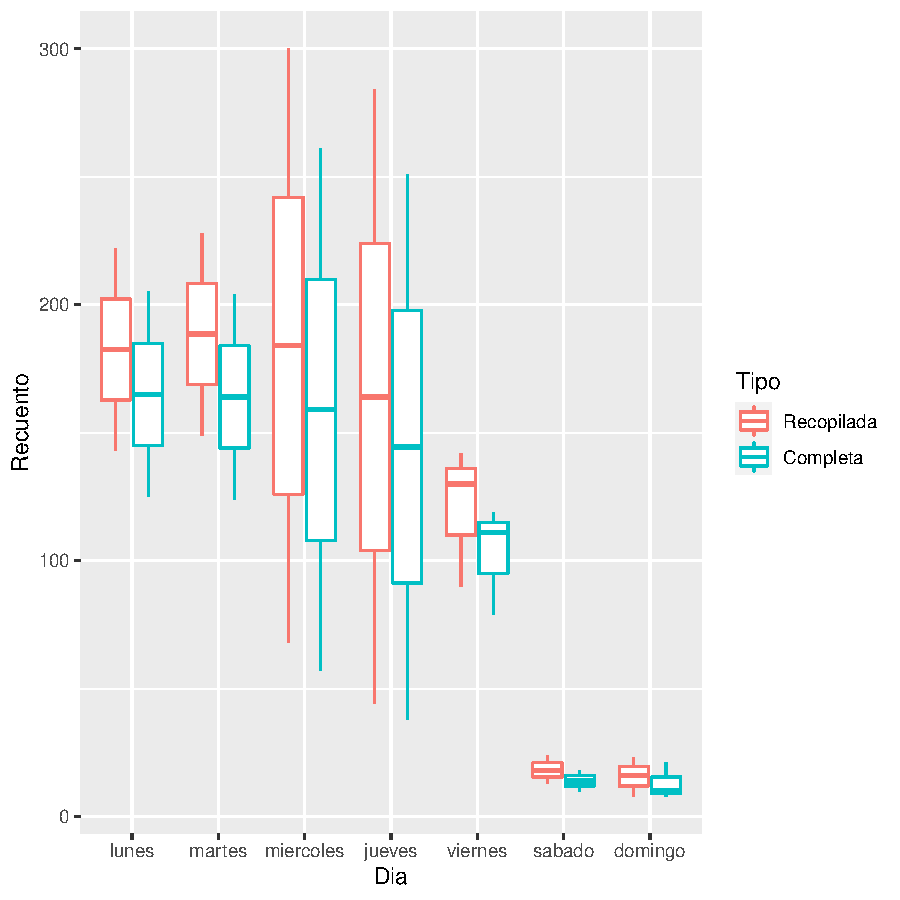
\includegraphics{seguimento2-026}

\subsection{Graficos de puntos}
Se mostraran las posibles relaciones entre las encuestas recopiladas y completas a lo largo del periodo 28 de febrero al 15 de marzo

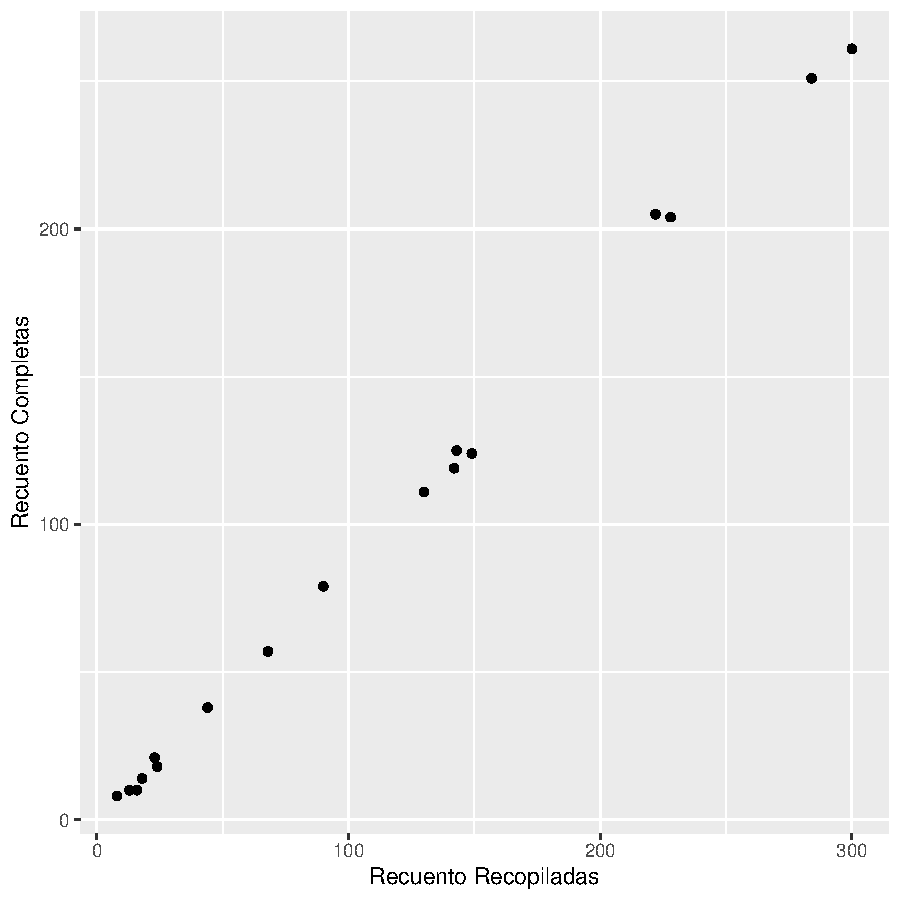
\includegraphics{seguimento2-027}

\subsubsection{Por meses}

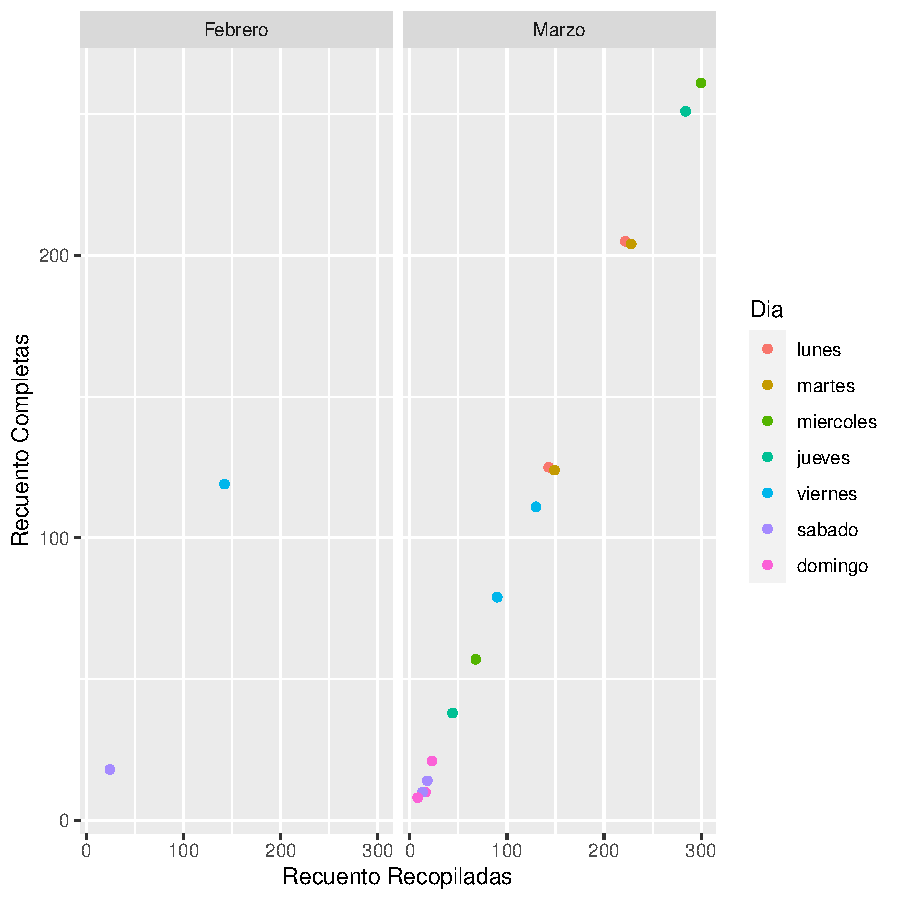
\includegraphics{seguimento2-028}

\subsubsection{Por dias}

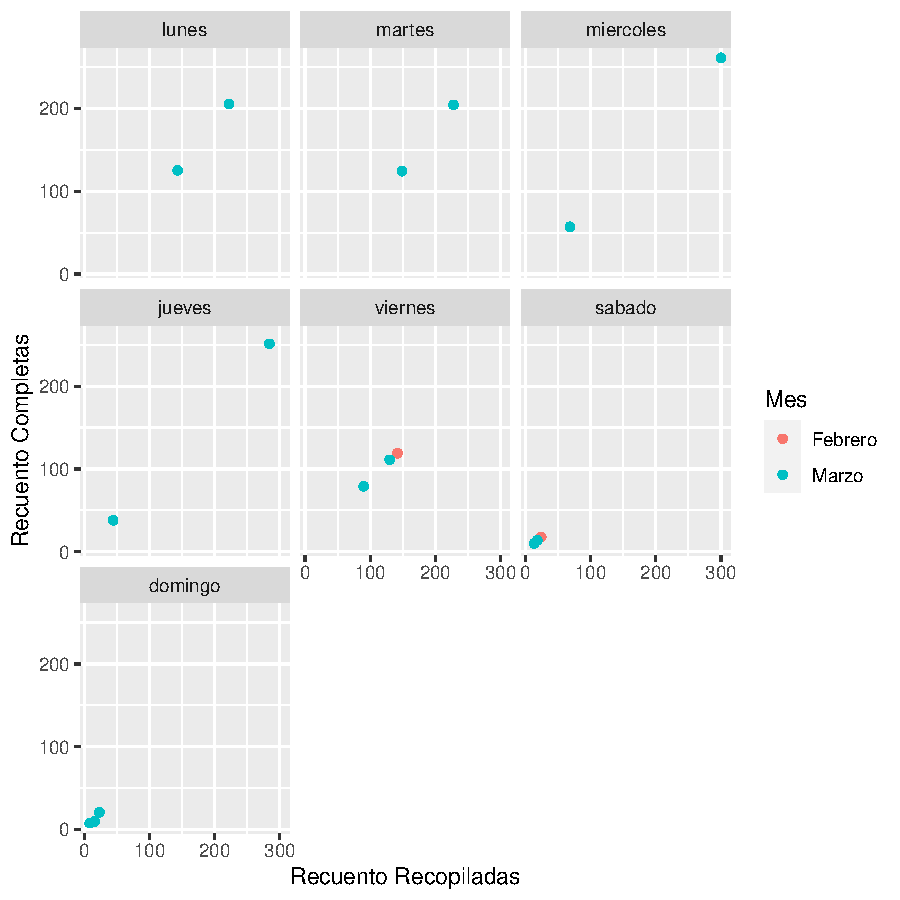
\includegraphics{seguimento2-029}

\section{Panorama despues del covid}
Esta etapa incluye desde el 16 de marzo hasta el 30 de junio

\subsection{Graficos de lineas}
Se muestran los cambios de la recoleccion de encuestas recopiladas y completas a lo largo del periodo 16 de marzo hasta el 30 de junio

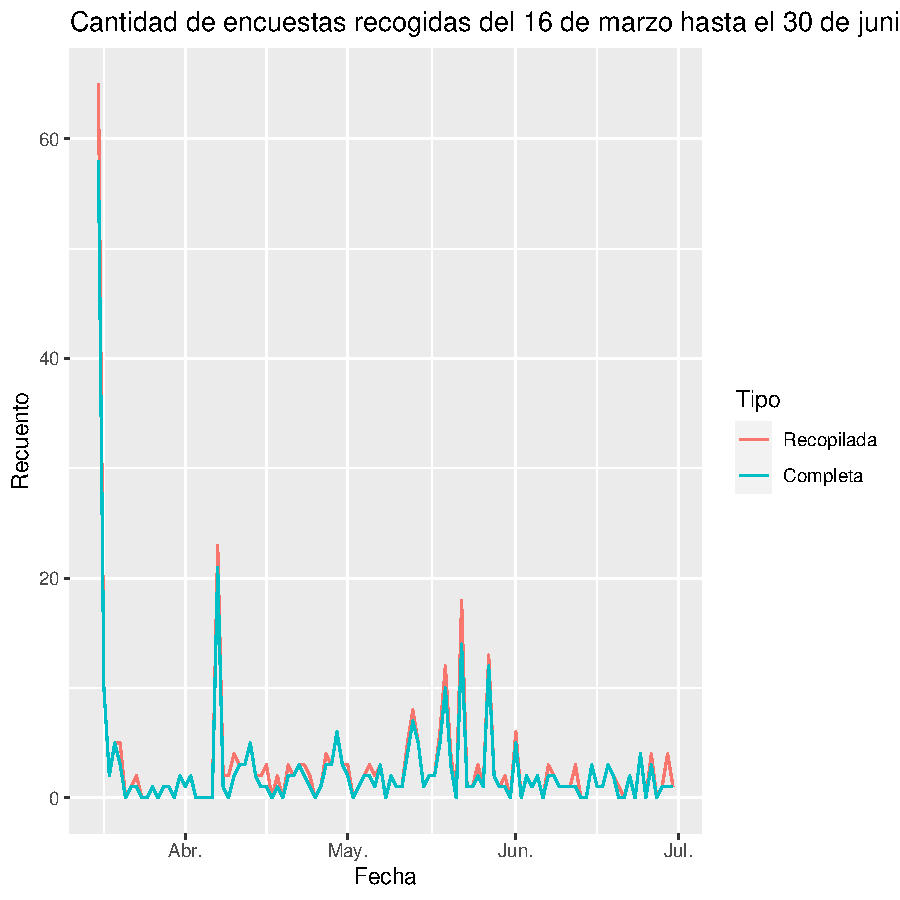
\includegraphics{seguimento2-030}

\subsection{Graficos de barras}
Se comparan las estadisticas de las encuestas recopiladas y completas a lo largo del periodo 16 de marzo hasta el 30 de junio

\begin{Schunk}
\begin{Soutput}
# A tibble: 2 x 4
  Tipo       minimo mediana maximo
  <fct>       <dbl>   <dbl>  <dbl>
1 Recopilada      0       2     65
2 Completa        0       1     58
\end{Soutput}
\end{Schunk}

\subsubsection{Minimo}

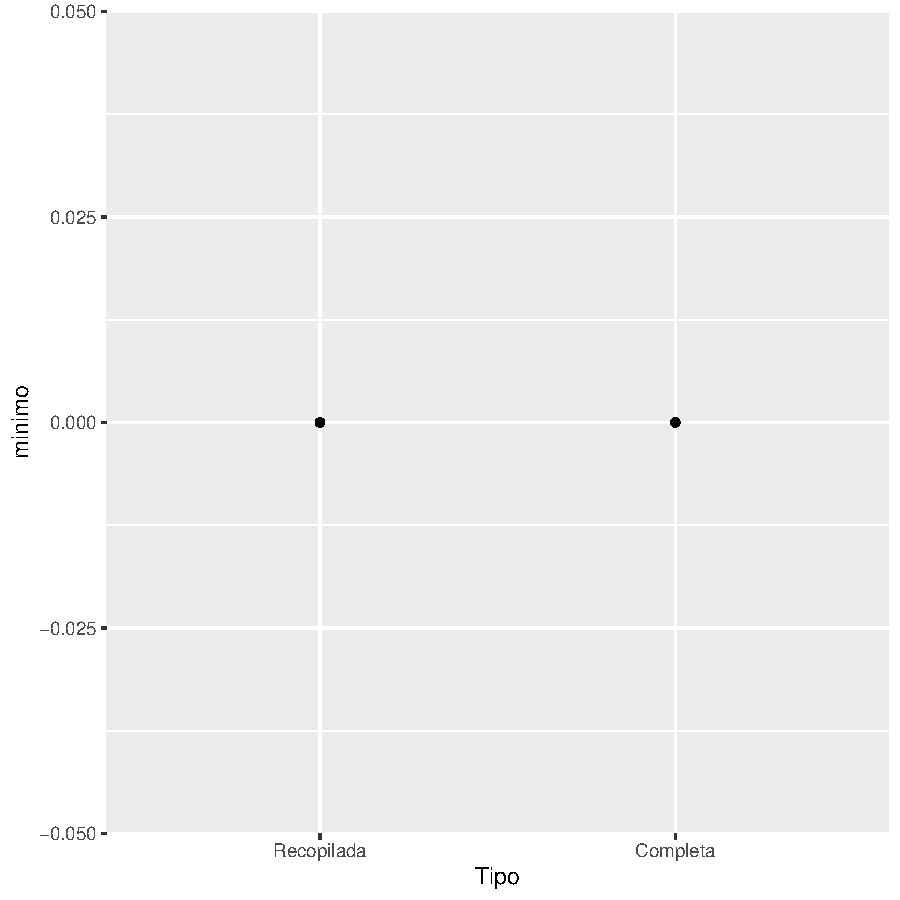
\includegraphics{seguimento2-032}

\subsubsection{Mediana}

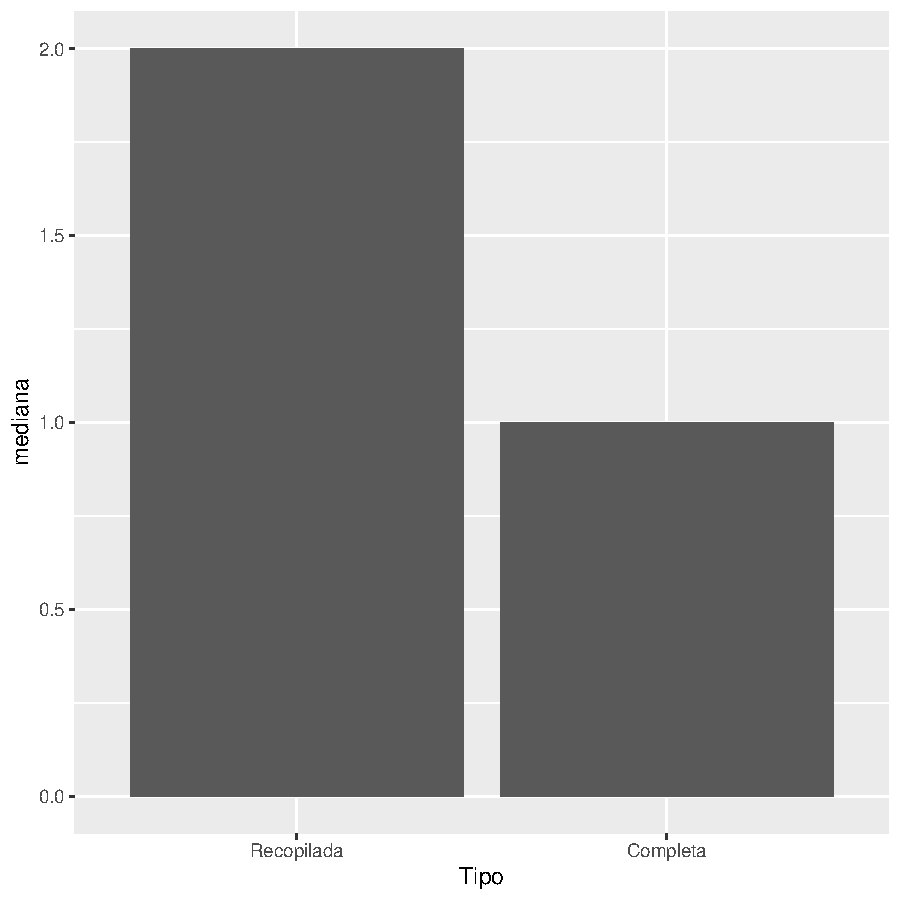
\includegraphics{seguimento2-033}

\subsubsection{Maximo}

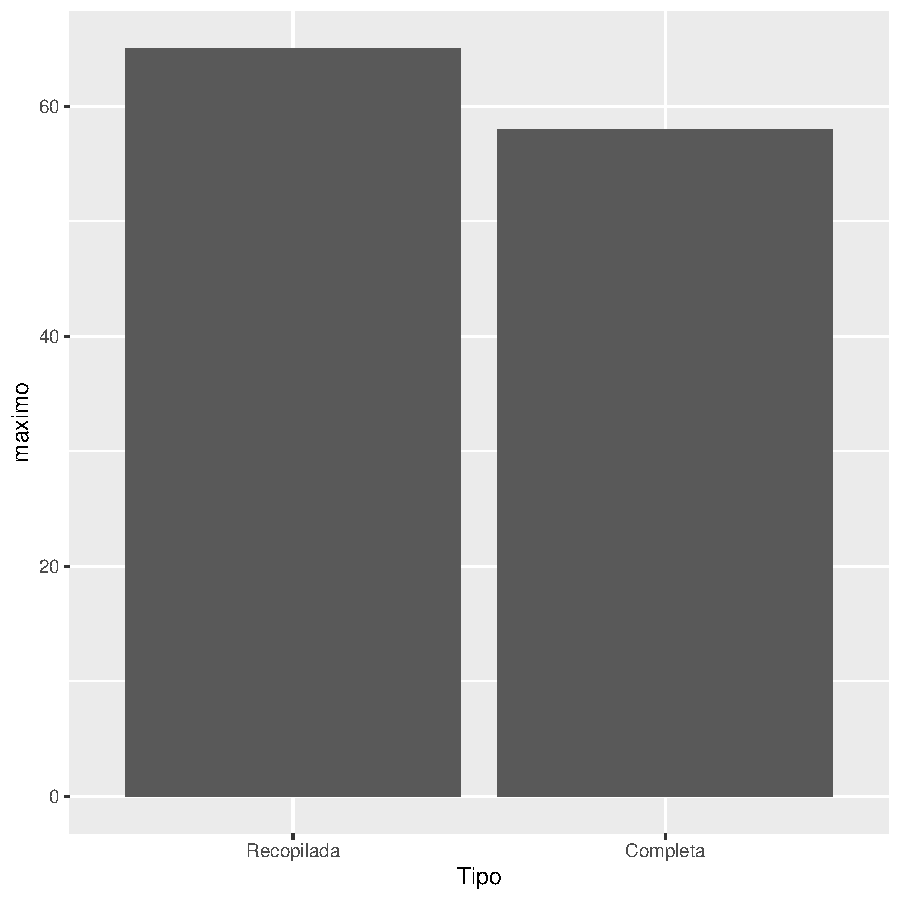
\includegraphics{seguimento2-034}

\subsection{Histogramas}
Se mostraran las distribuciones de las encuestas recopiladas y completas a lo largo del periodo 16 de marzo hasta el 30 de junio

\subsubsection{Recopilada}

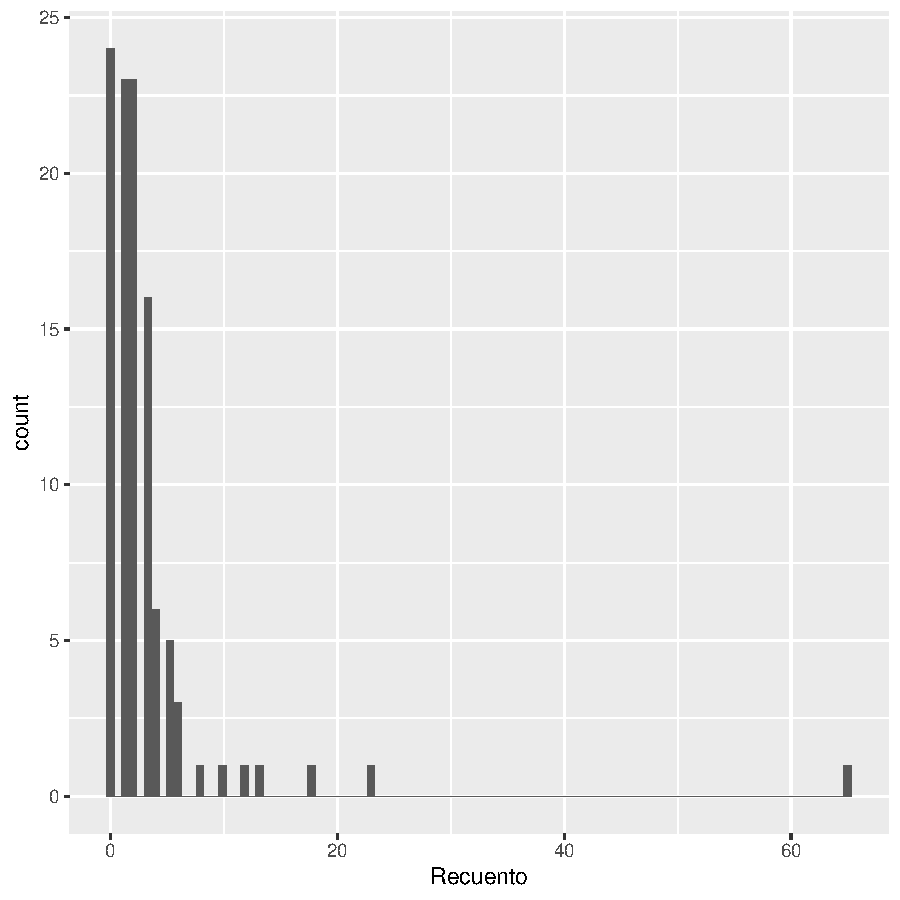
\includegraphics{seguimento2-035}


\subsubsection{Completa}

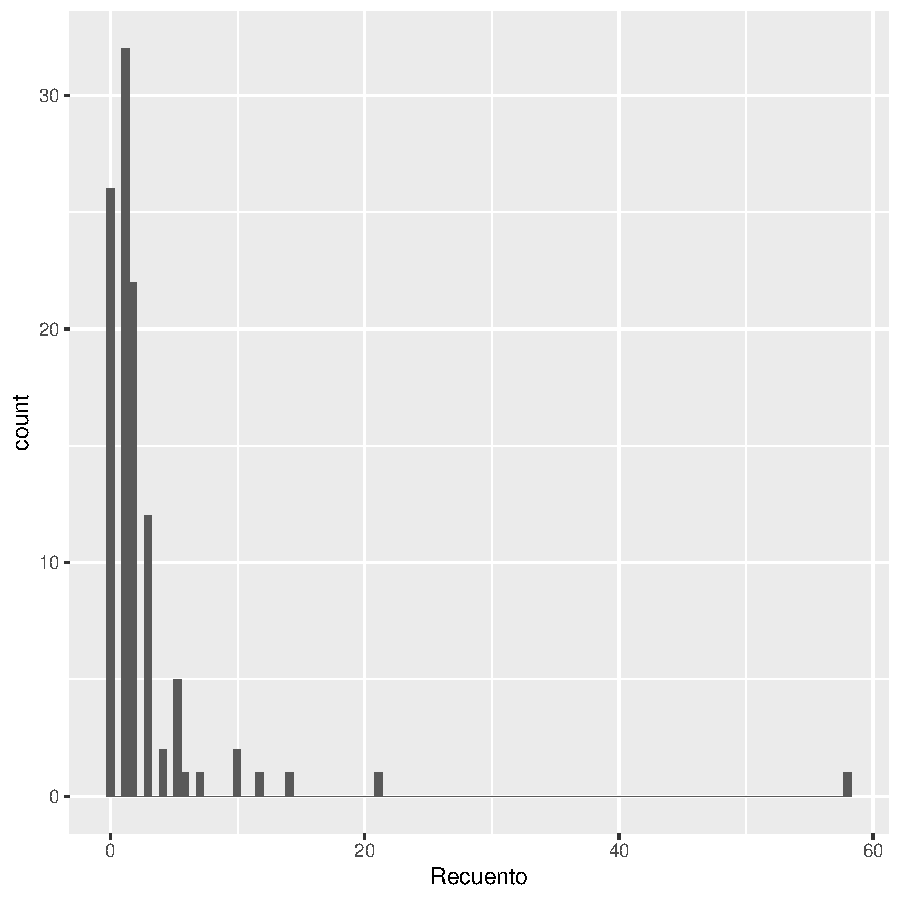
\includegraphics{seguimento2-036}

\subsection{Graficos de cajas}
Se comparan las distribuciones de las encuestas recopiladas y completas a lo largo del periodo 16 de marzo hasta el 30 de junio

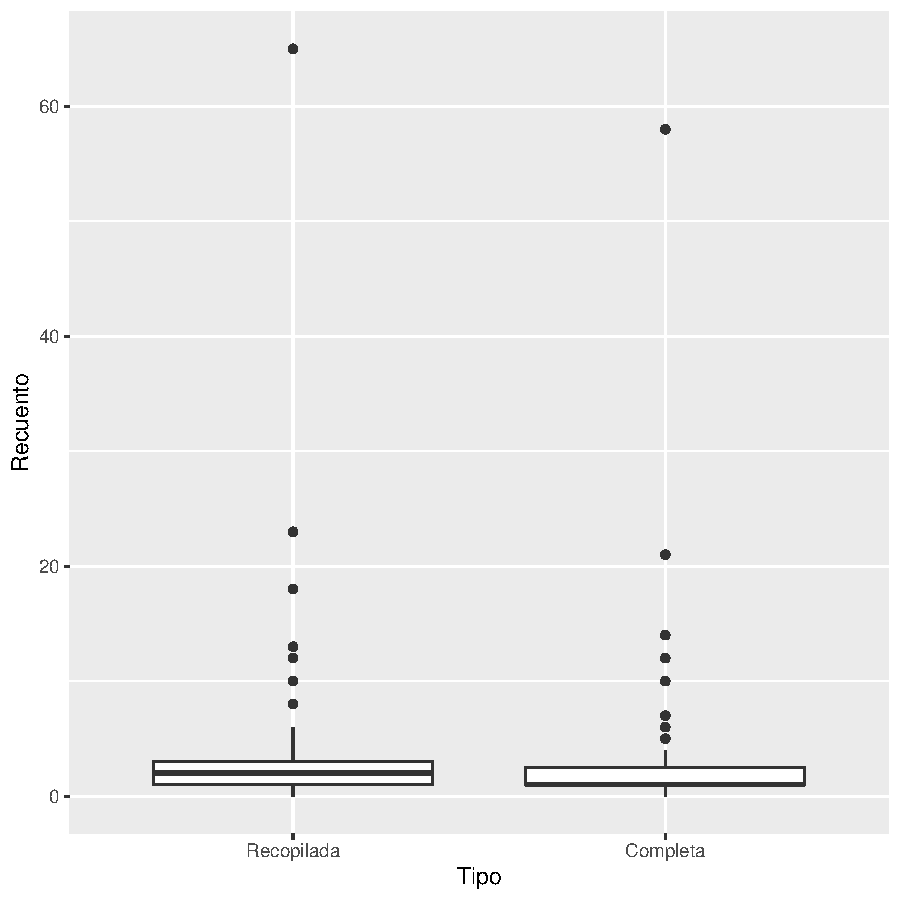
\includegraphics{seguimento2-037}

\subsubsection{Por meses}

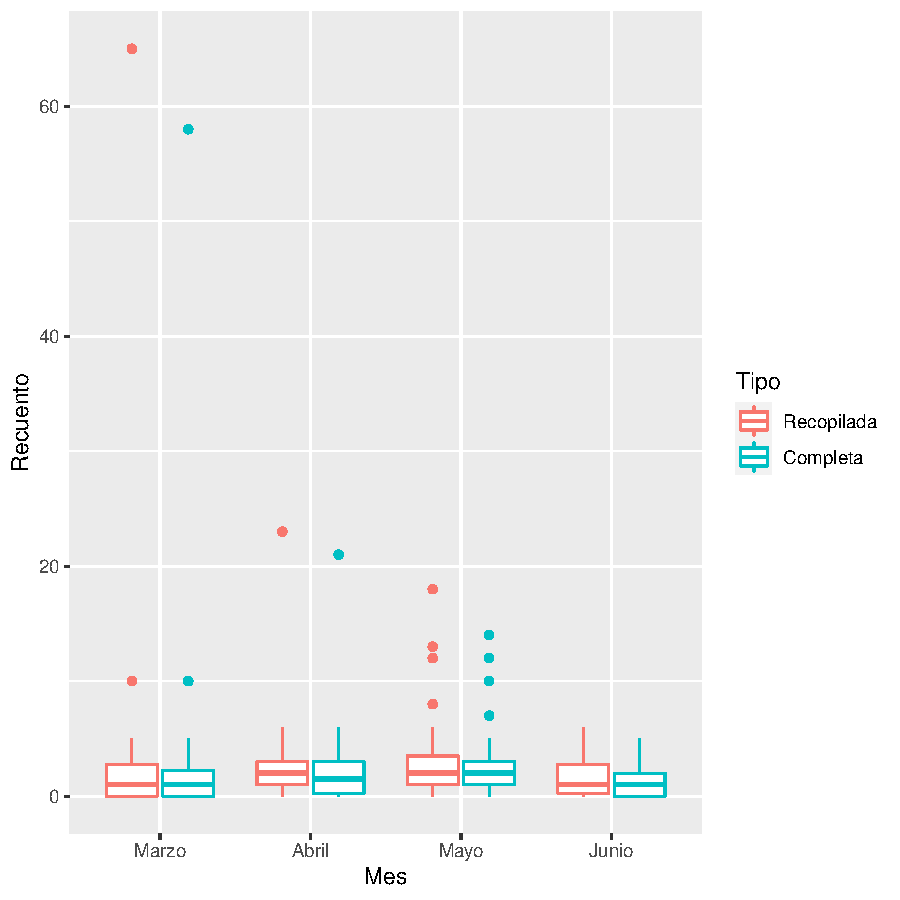
\includegraphics{seguimento2-038}

\subsubsection{Por dia de la semana}

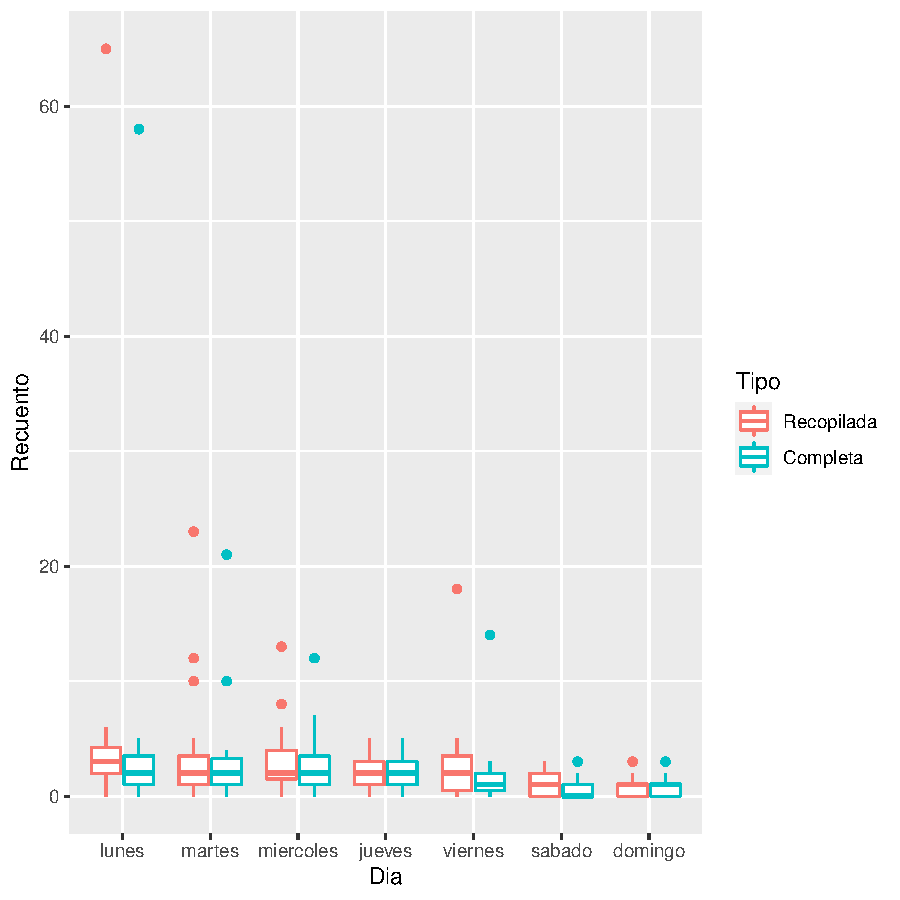
\includegraphics{seguimento2-039}

\subsection{Graficos de puntos}
Se mostraran las posibles relaciones entre las encuestas recopiladas y completas a lo largo del periodo 16 de marzo hasta el 30 de junio

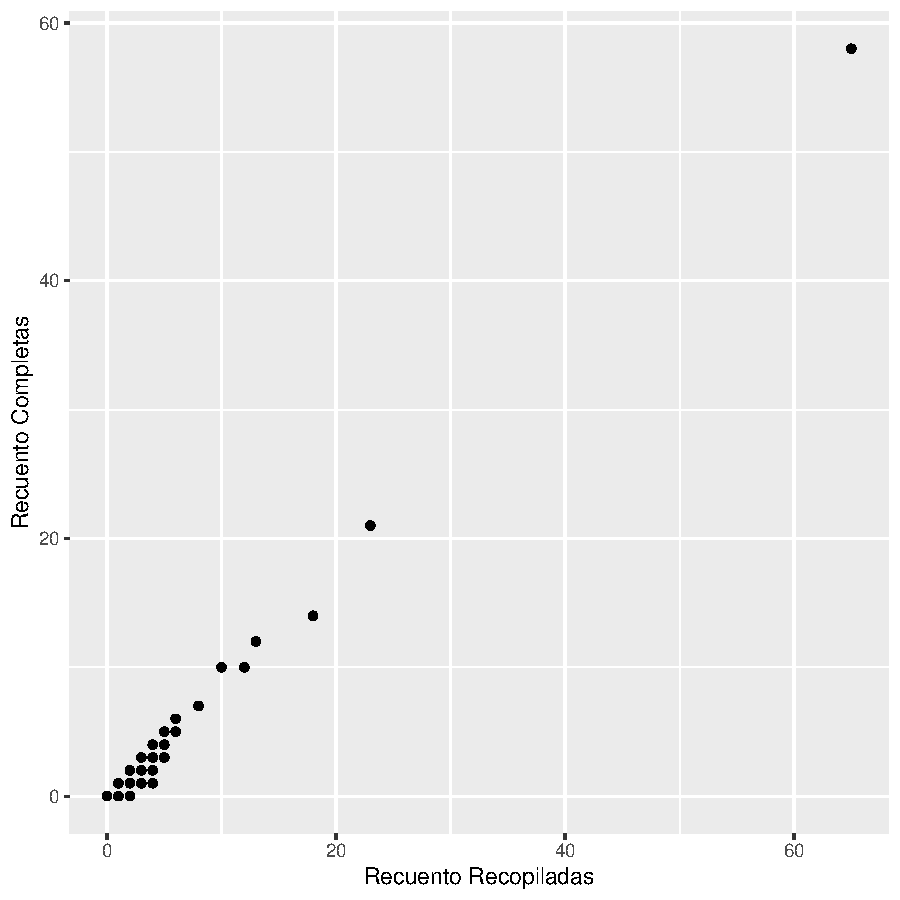
\includegraphics{seguimento2-040}

\subsubsection{Por meses}

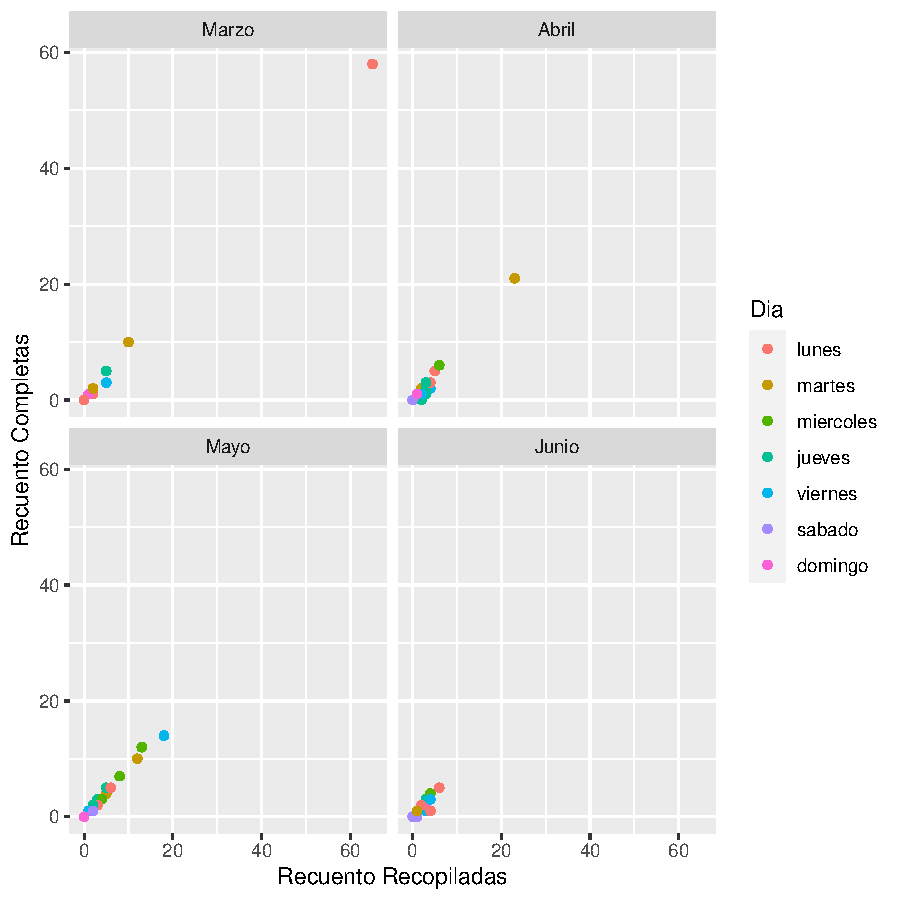
\includegraphics{seguimento2-041}

\subsubsection{Por dias}

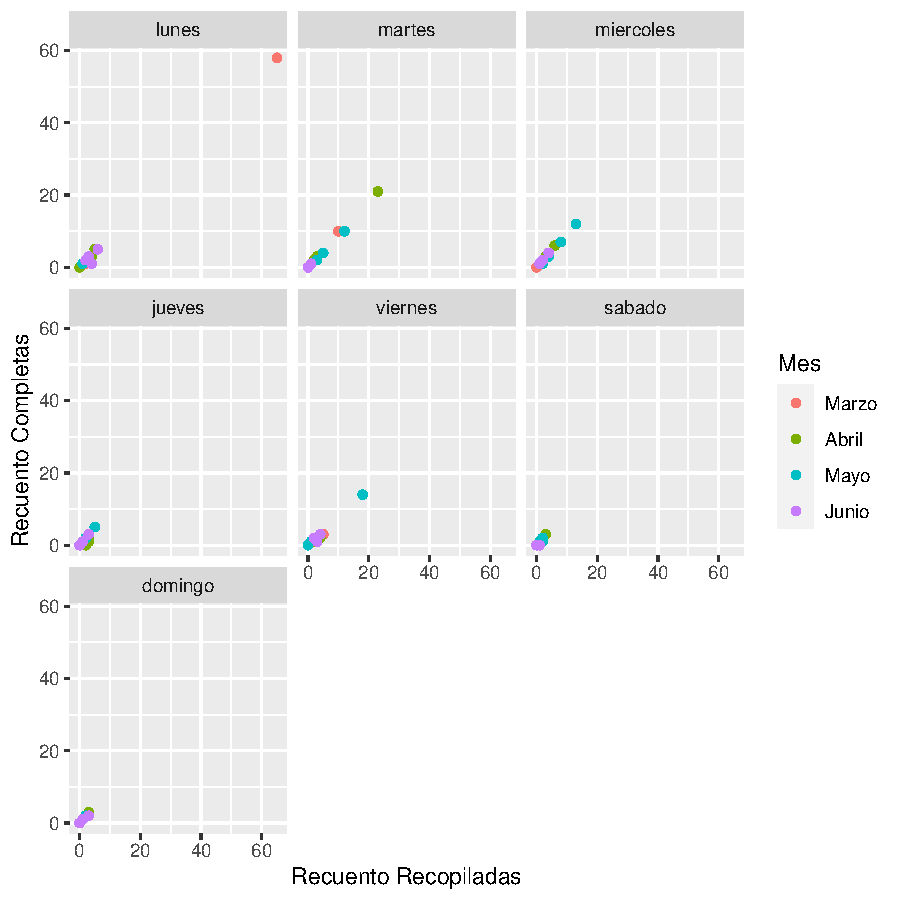
\includegraphics{seguimento2-042}

\section{Febrero}
El mes de febrero solo tuvo dos eventos que son el viernes 28 y el sabado 29, por lo cual se le discutira brevemente.

\subsection{Grafico de Columnas}
Compararemos los recuemtos que hubo esos dos dias

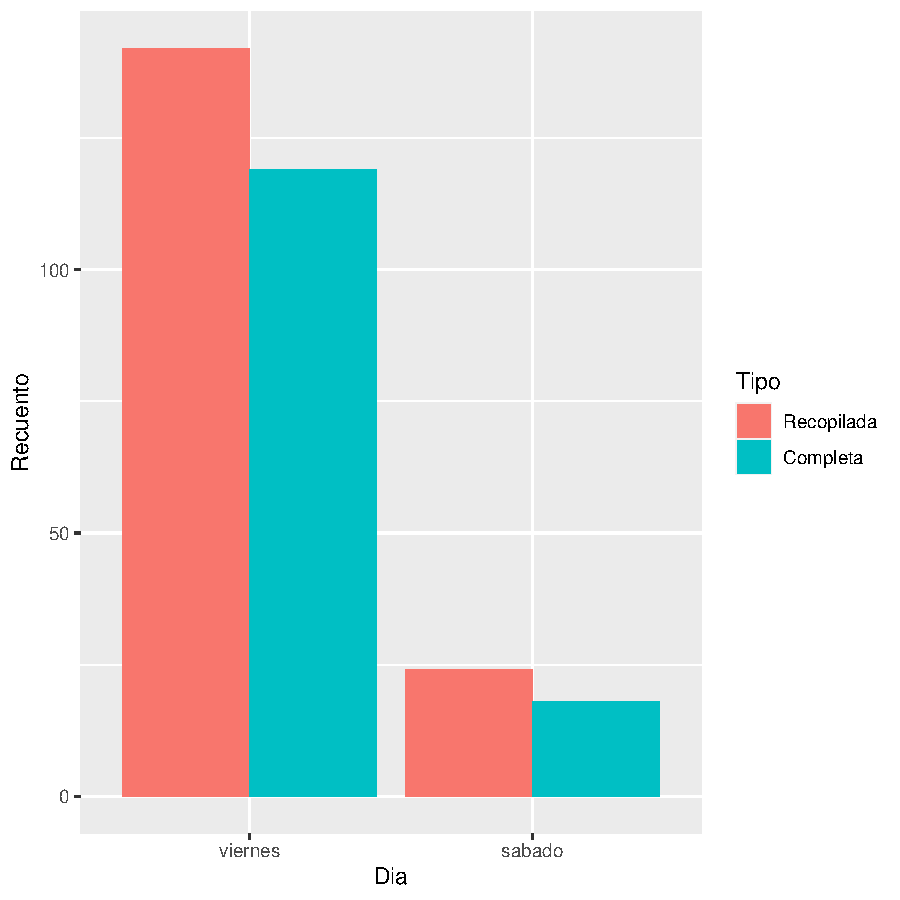
\includegraphics{seguimento2-043}

\section{Marzo antes del covid}
Esta etapa incluye desde el 1 de marzo hasta el 15 de marzo

\subsection{Graficos de lineas}
Se muestran los cambios de la recoleccion de encuestas recopiladas y completas a lo largo del periodo 1 de marzo hasta el 15 de marzo

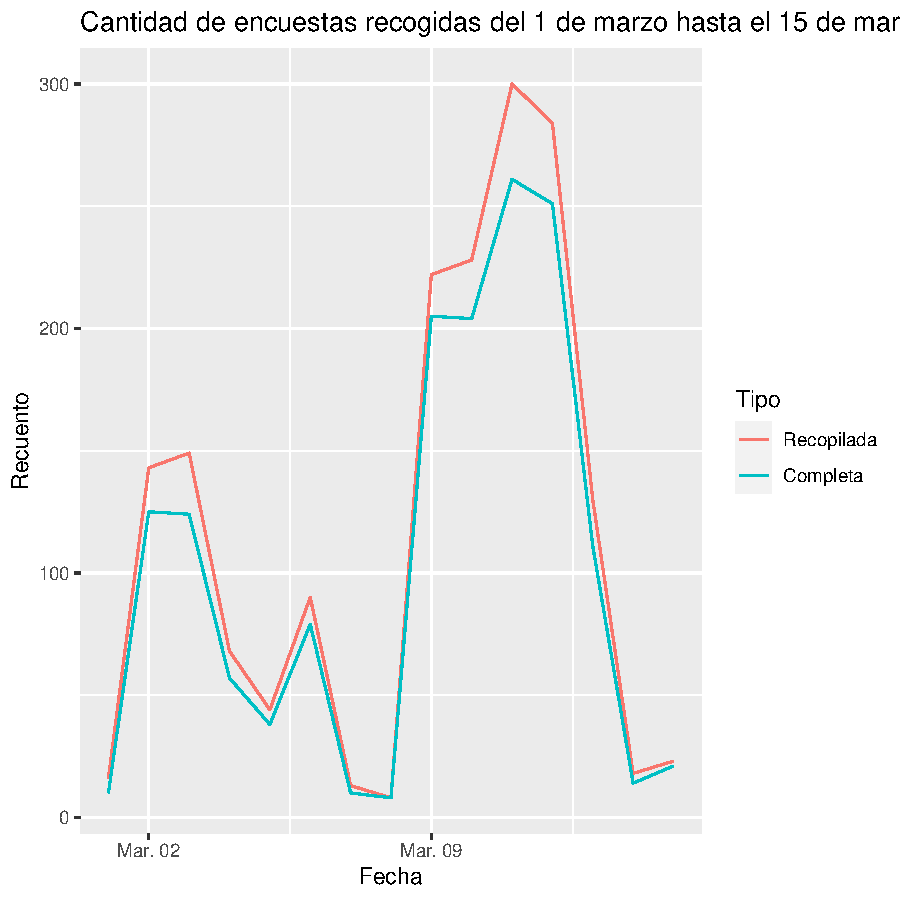
\includegraphics{seguimento2-044}

\subsection{Graficos de barras}
Se comparan las estadisticas de las encuestas recopiladas y completas a lo largo del periodo 1 de marzo hasta el 15 de marzo

\begin{Schunk}
\begin{Soutput}
# A tibble: 2 x 4
  Tipo       minimo mediana maximo
  <fct>       <dbl>   <dbl>  <dbl>
1 Recopilada      8      90    300
2 Completa        8      79    261
\end{Soutput}
\end{Schunk}

\subsubsection{Minimo}

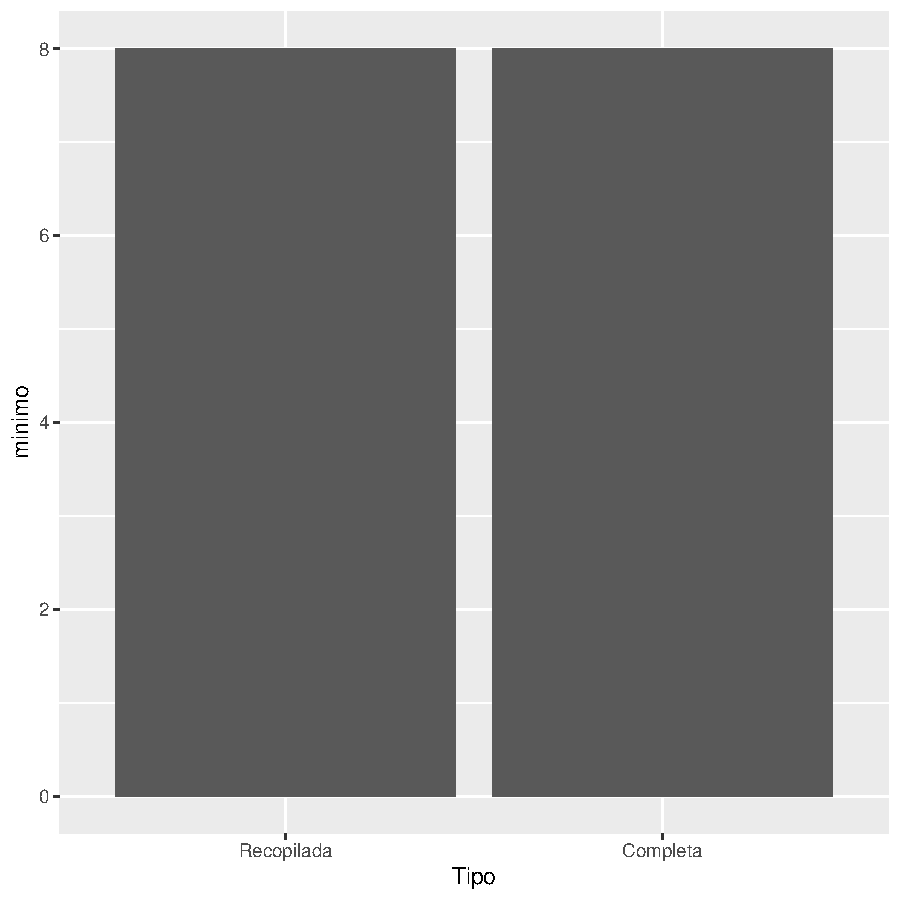
\includegraphics{seguimento2-046}

\subsubsection{Mediana}

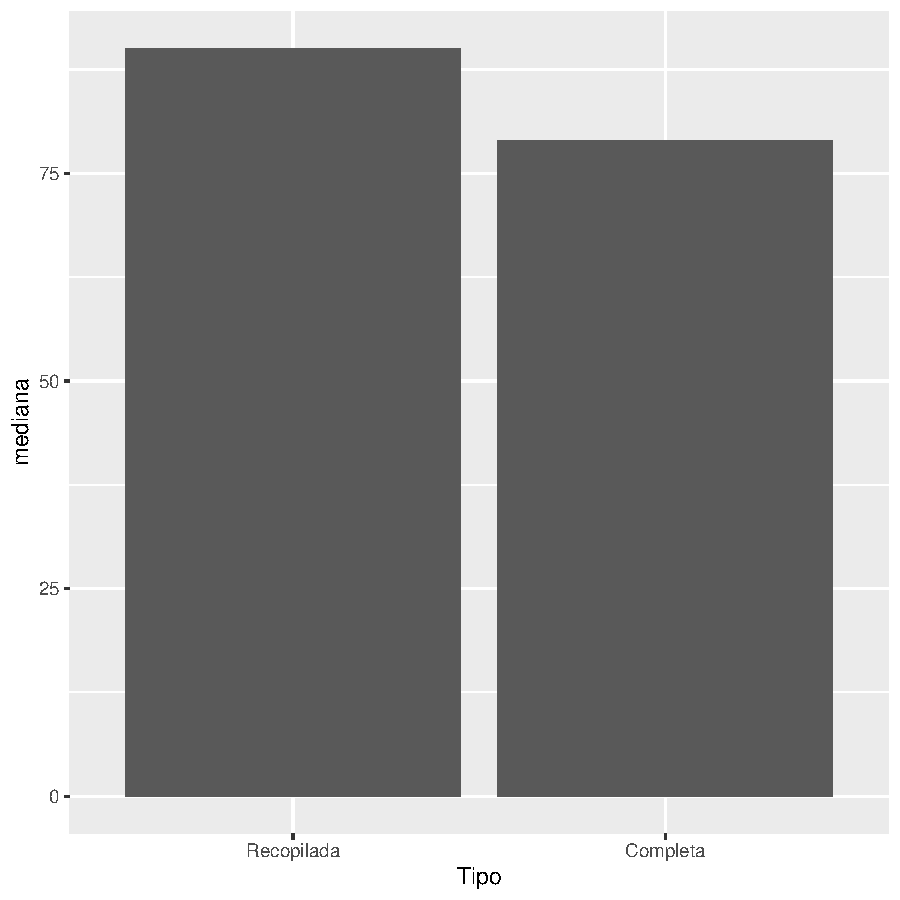
\includegraphics{seguimento2-047}

\subsubsection{Maximo}

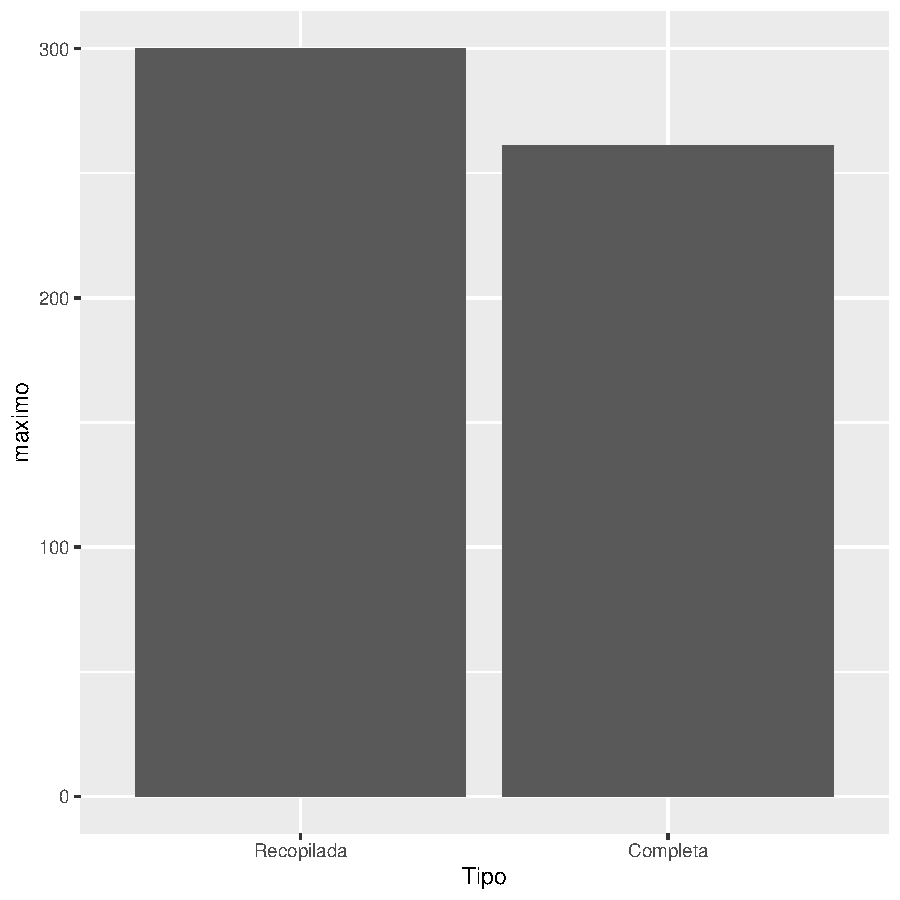
\includegraphics{seguimento2-048}

\subsection{Histogramas}
Se mostraran las distribuciones de las encuestas recopiladas y completas a lo largo del periodo 1 de marzo hasta el 15 de marzo

\subsubsection{Recopilada}

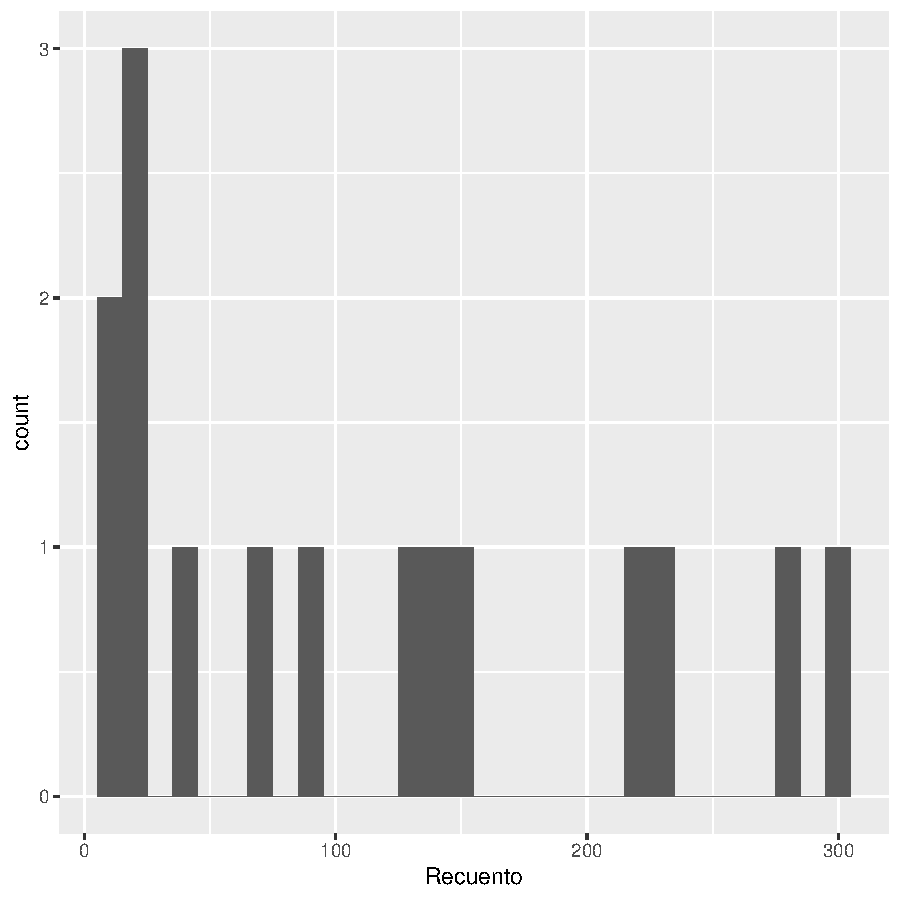
\includegraphics{seguimento2-049}


\subsubsection{Completa}

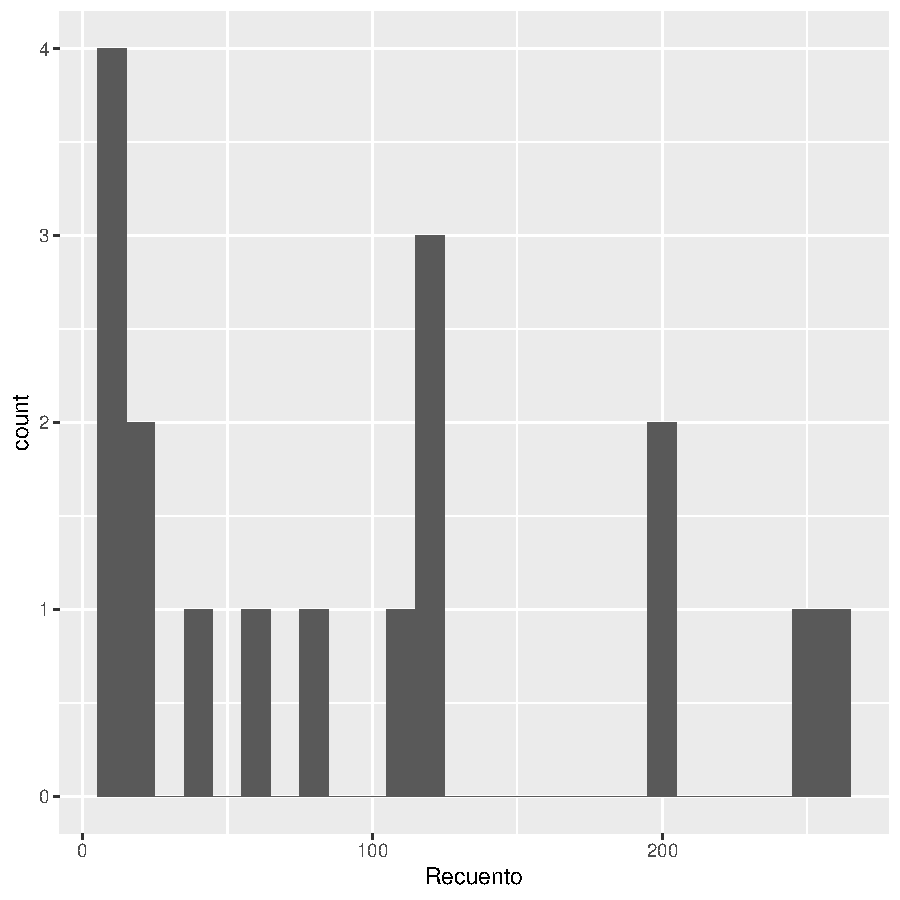
\includegraphics{seguimento2-050}

\subsection{Graficos de cajas}
Se comparan las distribuciones de las encuestas recopiladas y completas a lo largo del periodo 1 de marzo hasta el 15 de marzo

\subsubsection{Marzo sin covid}

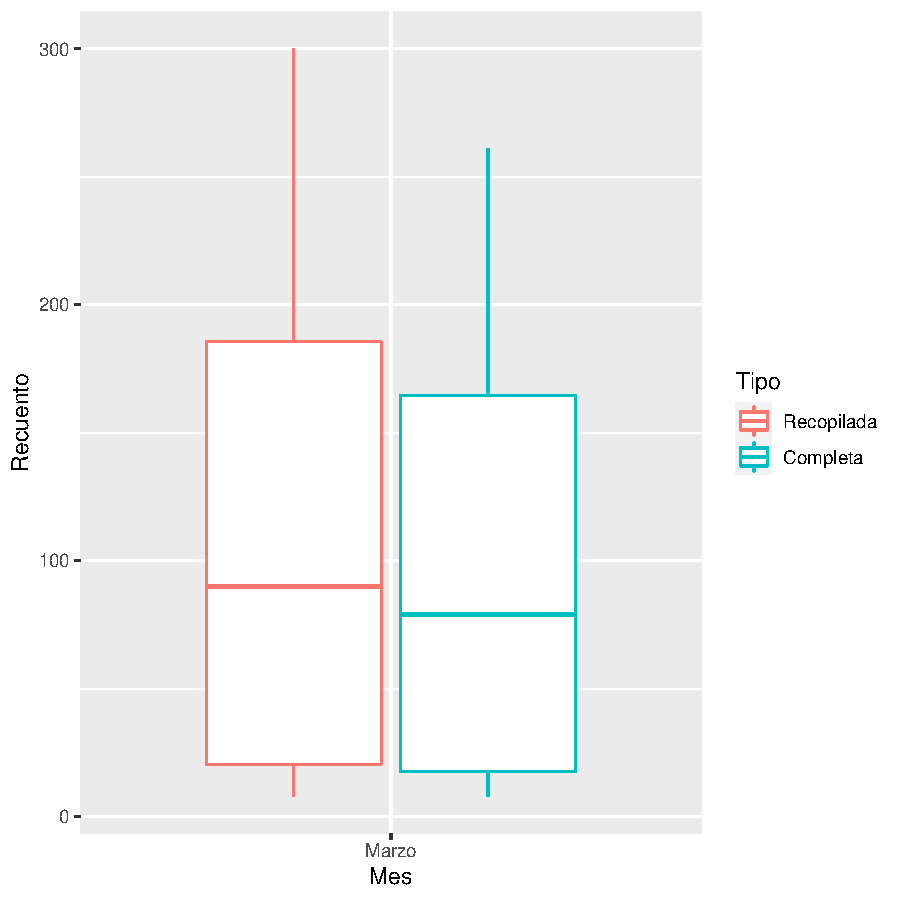
\includegraphics{seguimento2-051}

\subsubsection{Por dia de la semana}

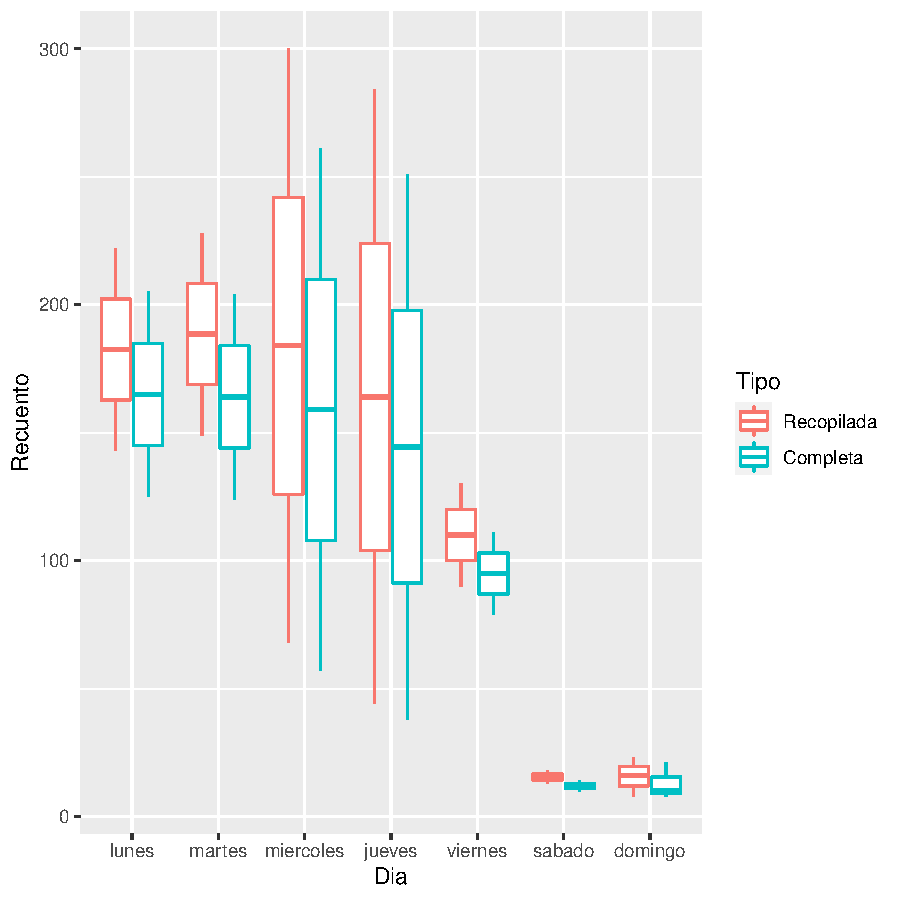
\includegraphics{seguimento2-052}

\subsection{Graficos de puntos}
Se mostraran las posibles relaciones entre las encuestas recopiladas y completas a lo largo del periodo 1 de marzo hasta el 17 de marzo

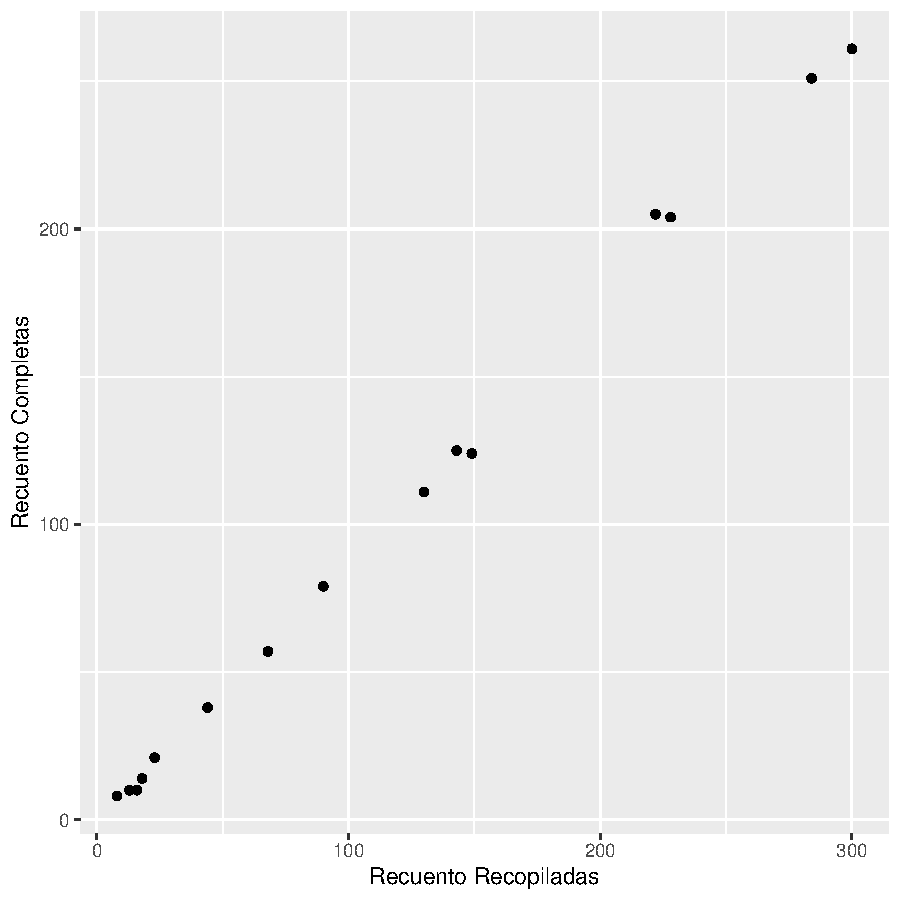
\includegraphics{seguimento2-053}

\subsubsection{Por dias}

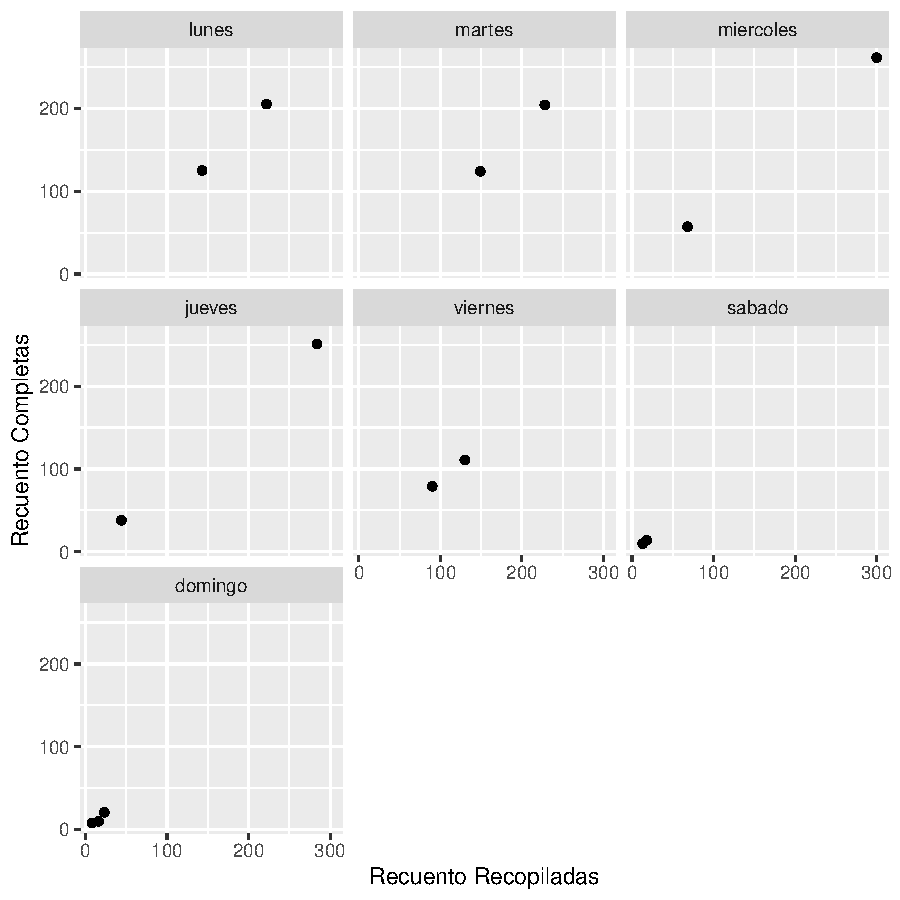
\includegraphics{seguimento2-054}

\section{Marzo despues del covid}
Esta etapa incluye desde el 16 de marzo hasta el 31 de marzo

\subsection{Graficos de lineas}
Se muestran los cambios de la recoleccion de encuestas recopiladas y completas a lo largo del periodo 16 de marzo hasta el 31 de marzo

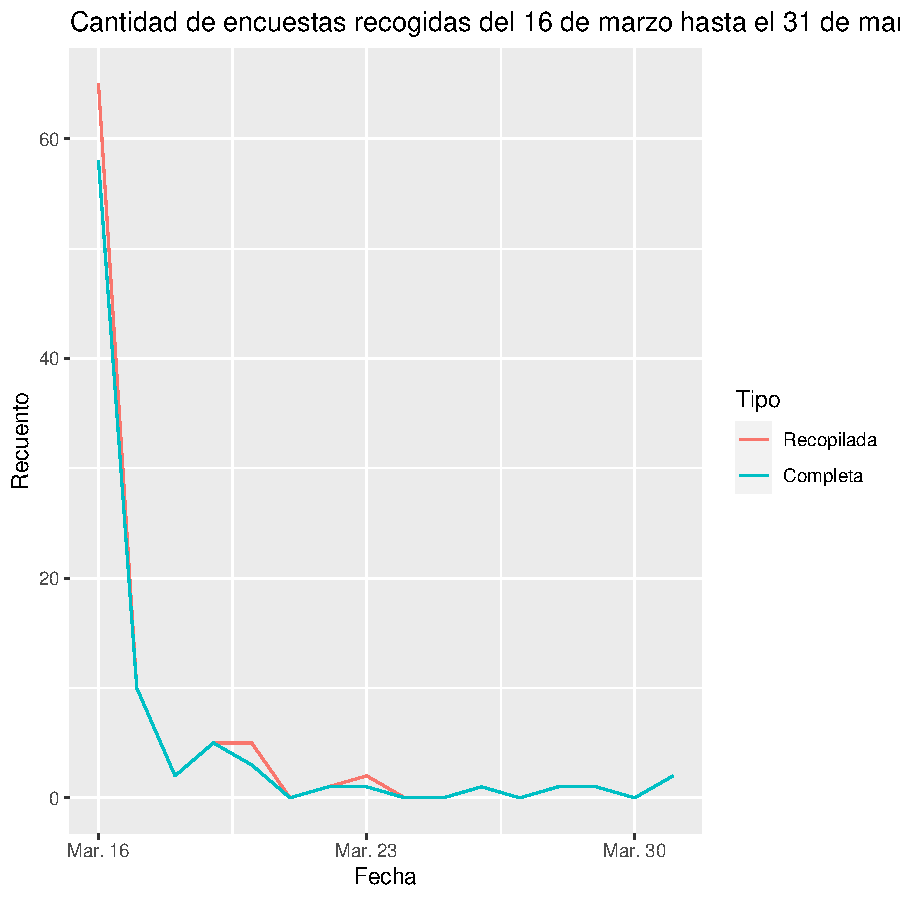
\includegraphics{seguimento2-055}

\subsection{Graficos de barras}
Se comparan las estadisticas de las encuestas recopiladas y completas a lo largo del periodo 16 de marzo hasta el 31 de marzo

\begin{Schunk}
\begin{Soutput}
# A tibble: 2 x 4
  Tipo       minimo mediana maximo
  <fct>       <dbl>   <dbl>  <dbl>
1 Recopilada      0       1     65
2 Completa        0       1     58
\end{Soutput}
\end{Schunk}

\subsubsection{Minimo}

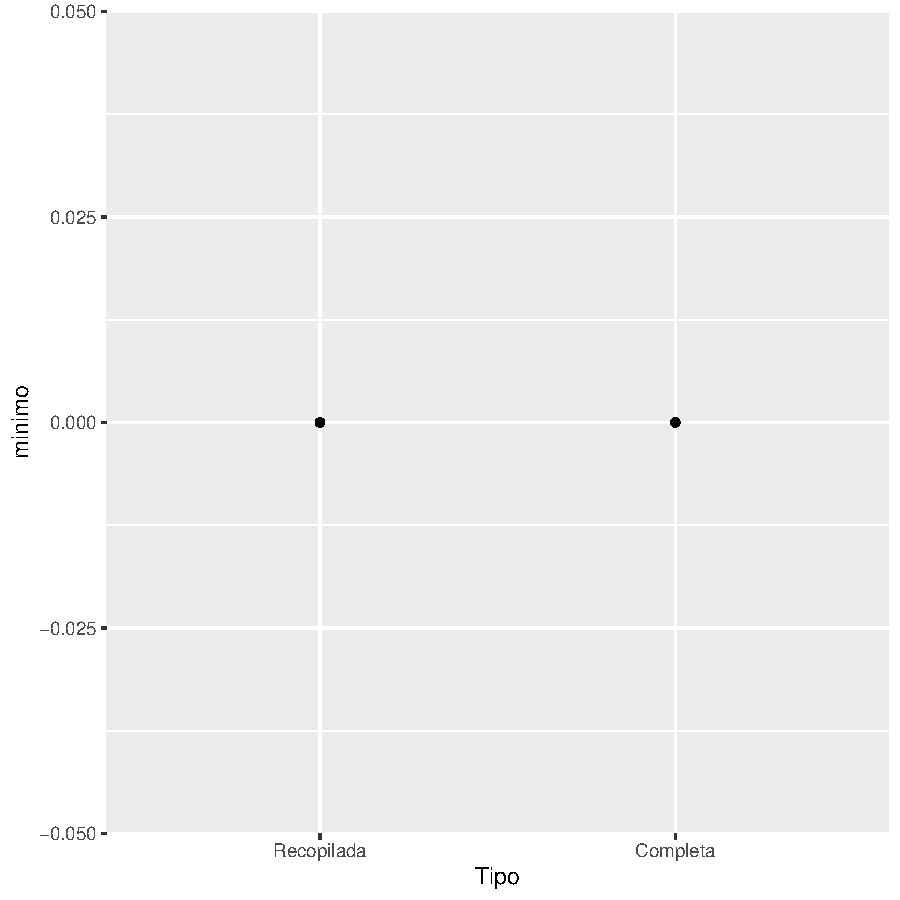
\includegraphics{seguimento2-057}

\subsubsection{Mediana}

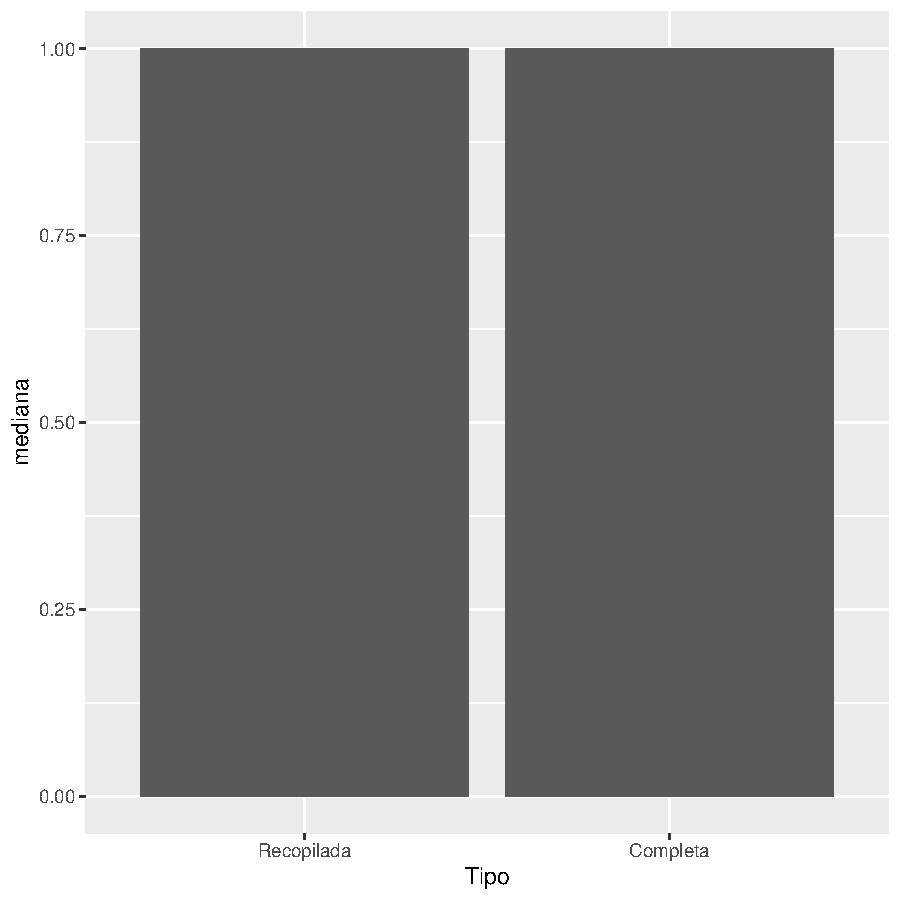
\includegraphics{seguimento2-058}

\subsubsection{Maximo}

\includegraphics{seguimento2-059}

\subsection{Histogramas}
Se mostraran las distribuciones de las encuestas recopiladas y completas a lo largo del periodo 16 de marzo hasta el 31 de marzo

\subsubsection{Recopilada}

\includegraphics{seguimento2-060}


\subsubsection{Completa}

\includegraphics{seguimento2-061}

\subsection{Graficos de cajas}
Se comparan las distribuciones de las encuestas recopiladas y completas a lo largo del periodo 16 de marzo hasta el 31 de marzo

\subsubsection{Marzo con covid}

\includegraphics{seguimento2-062}

\subsubsection{Por dia de la semana}

\includegraphics{seguimento2-063}

\subsection{Graficos de puntos}
Se mostraran las posibles relaciones entre las encuestas recopiladas y completas a lo largo del periodo 16 de marzo hasta el 31 de marzo

\includegraphics{seguimento2-064}

\subsubsection{Por dias}

\includegraphics{seguimento2-065}

\section{Abril}
\subsection{Graficos de lineas}
Se muestran los cambios de la recoleccion de encuestas recopiladas y completas a lo largo del periodo de Abril

\includegraphics{seguimento2-066}

\subsection{Graficos de barras}
Se comparan las estadisticas de las encuestas recopiladas y completas a lo largo del periodo de Abril

\begin{Schunk}
\begin{Soutput}
# A tibble: 2 x 4
  Tipo       minimo mediana maximo
  <fct>       <dbl>   <dbl>  <dbl>
1 Recopilada      0     2       23
2 Completa        0     1.5     21
\end{Soutput}
\end{Schunk}

\subsubsection{Minimo}
El valor es de cero para recopiladas y completas

\includegraphics{seguimento2-068}

\subsubsection{Mediana}

\includegraphics{seguimento2-069}

\subsubsection{Maximo}

\includegraphics{seguimento2-070}

\subsection{Histogramas}
Se mostraran las distribuciones de las encuestas recopiladas y completas a lo largo del periodo de Abril

\subsubsection{Recopilada}

\includegraphics{seguimento2-071}

\subsubsection{Completa}

\includegraphics{seguimento2-072}

\subsection{Graficos de cajas}
Se comparan las distribuciones de las encuestas recopiladas y completas a lo largo del periodo de Abril

\subsubsection{Abril}

\includegraphics{seguimento2-073}

\subsubsection{Por dia de la semana}

\includegraphics{seguimento2-074}

\subsection{Graficos de puntos}
Se mostraran las posibles relaciones entre las encuestas recopiladas y completas a lo largo del periodo de Abril

\includegraphics{seguimento2-075}


\subsubsection{Por dias}

\includegraphics{seguimento2-076}

\section{Mayo}
\subsection{Graficos de lineas}
Se muestran los cambios de la recoleccion de encuestas recopiladas y completas a lo largo del periodo de Mayo

\includegraphics{seguimento2-077}

\subsection{Graficos de barras}
Se comparan las estadisticas de las encuestas recopiladas y completas a lo largo del periodo de Mayo

\begin{Schunk}
\begin{Soutput}
# A tibble: 2 x 4
  Tipo       minimo mediana maximo
  <fct>       <dbl>   <dbl>  <dbl>
1 Recopilada      0       2     18
2 Completa        0       2     14
\end{Soutput}
\end{Schunk}

\subsubsection{Minimo}
El valor es de cero para recopiladas y completas

\includegraphics{seguimento2-079}

\subsubsection{Mediana}

\includegraphics{seguimento2-080}

\subsubsection{Maximo}

\includegraphics{seguimento2-081}

\subsection{Histogramas}
Se mostraran las distribuciones de las encuestas recopiladas y completas a lo largo del periodo de Mayo

\subsubsection{Recopilada}

\includegraphics{seguimento2-082}

\subsubsection{Completa}

\includegraphics{seguimento2-083}

\subsection{Graficos de cajas}
Se comparan las distribuciones de las encuestas recopiladas y completas a lo largo del periodo de Mayo

\subsubsection{Mayo}

\includegraphics{seguimento2-084}

\subsubsection{Por dia de la semana}

\includegraphics{seguimento2-085}

\subsection{Graficos de puntos}
Se mostraran las posibles relaciones entre las encuestas recopiladas y completas a lo largo del periodo de Mayo

\includegraphics{seguimento2-086}


\subsubsection{Por dias}

\includegraphics{seguimento2-087}

\section{Junio}
\subsection{Graficos de lineas}
Se muestran los cambios de la recoleccion de encuestas recopiladas y completas a lo largo del periodo de Junio

\includegraphics{seguimento2-088}

\subsection{Graficos de barras}
Se comparan las estadisticas de las encuestas recopiladas y completas a lo largo del periodo de Junio

\begin{Schunk}
\begin{Soutput}
# A tibble: 2 x 4
  Tipo       minimo mediana maximo
  <fct>       <dbl>   <dbl>  <dbl>
1 Recopilada      0       1      6
2 Completa        0       1      5
\end{Soutput}
\end{Schunk}

\subsubsection{Minimo}
El valor es de cero para recopiladas y completas

\includegraphics{seguimento2-090}

\subsubsection{Mediana}

\includegraphics{seguimento2-091}

\subsubsection{Maximo}

\includegraphics{seguimento2-092}

\subsection{Histogramas}
Se mostraran las distribuciones de las encuestas recopiladas y completas a lo largo del periodo de Junio

\subsubsection{Recopilada}

\includegraphics{seguimento2-093}

\subsubsection{Completa}

\includegraphics{seguimento2-094}

\subsection{Graficos de cajas}
Se comparan las distribuciones de las encuestas recopiladas y completas a lo largo del periodo de Junio

\subsubsection{Junio}

\includegraphics{seguimento2-095}

\subsubsection{Por dia de la semana}

\includegraphics{seguimento2-096}

\subsection{Graficos de puntos}
Se mostraran las posibles relaciones entre las encuestas recopiladas y completas a lo largo del periodo de Junio

\includegraphics{seguimento2-097}

\subsubsection{Por dias}

\includegraphics{seguimento2-098}


\end{document}
